%!TEX TS-program = xelatex
\documentclass[12pt, a4paper, oneside]{article}

% пакеты для математики
\usepackage{amsmath,amsfonts,amssymb,amsthm,mathtools}  
\mathtoolsset{showonlyrefs=true}  % Показывать номера только у тех формул, на которые есть \eqref{} в тексте.

\usepackage[english, russian]{babel} % выбор языка для документа
% \usepackage[utf8]{inputenc}          % utf8 кодировка

% Основные шрифты 
\usepackage{fontspec}         
\setmainfont{Linux Libertine O}  % задаёт основной шрифт документа

% Математические шрифты 
\usepackage{unicode-math}     
\setmathfont[math-style=upright]{[Neo Euler.otf]} 


%%%%%%%%%% Работа с картинками и таблицами %%%%%%%%%%
\usepackage{graphicx} % Для вставки рисунков                
\usepackage{graphics}
\graphicspath{{images/}{pictures/}}   % папки с картинками

\usepackage{wrapfig}    % обтекание рисунков и таблиц текстом

\usepackage{booktabs}   % таблицы как в годных книгах
\usepackage{tabularx}   % новые типы колонок
\usepackage{tabulary}   % и ещё новые типы колонок
\usepackage{float}      % возможность позиционировать объекты в нужном месте
\renewcommand{\arraystretch}{1.2}  % больше расстояние между строками


%%%%%%%%%% Графики и рисование %%%%%%%%%%
\usepackage{tikz, pgfplots}  % языки для графики
\pgfplotsset{compat=1.16}

\usepackage{todonotes} % для вставки в документ заметок о том, что осталось сделать
% \todo{Здесь надо коэффициенты исправить}
% \missingfigure{Здесь будет Последний день Помпеи}
% \listoftodos --- печатает все поставленные \todo'шки


%%%%%%%%%% Внешний вид страницы %%%%%%%%%%

\usepackage[paper=a4paper, top=20mm, bottom=15mm,left=20mm,right=15mm]{geometry}
\usepackage{indentfirst}    % установка отступа в первом абзаце главы

\usepackage{setspace}
\setstretch{1.15}  % межстрочный интервал
\setlength{\parskip}{4mm}   % Расстояние между абзацами
% Разные длины в LaTeX: https://en.wikibooks.org/wiki/LaTeX/Lengths

% свешиваем пунктуацию
% теперь знаки пунктуации могут вылезать за правую границу текста, при этом текст выглядит ровнее
\usepackage{microtype}

% \flushbottom                            % Эта команда заставляет LaTeX чуть растягивать строки, чтобы получить идеально прямоугольную страницу
\righthyphenmin=2                       % Разрешение переноса двух и более символов
\widowpenalty=300                     % Небольшое наказание за вдовствующую строку (одна строка абзаца на этой странице, остальное --- на следующей)
\clubpenalty=3000                     % Приличное наказание за сиротствующую строку (омерзительно висящая одинокая строка в начале страницы)
\tolerance=10000     % Ещё какое-то наказание.

% мои цвета https://www.artlebedev.ru/colors/
\definecolor{titleblue}{rgb}{0.2,0.4,0.6} 
\definecolor{blue}{rgb}{0.2,0.4,0.6} 
\definecolor{red}{rgb}{1,0,0.2} 
\definecolor{green}{rgb}{0,0.6,0} 
\definecolor{purp}{rgb}{0.4,0,0.8} 

% цвета из geogebra 
\definecolor{litebrown}{rgb}{0.6,0.2,0}
\definecolor{darkbrown}{rgb}{0.75,0.75,0.75}

% Гиперссылки
\usepackage{xcolor}   % разные цвета

\usepackage{hyperref}
\hypersetup{
	unicode=true,           % позволяет использовать юникодные символы
	colorlinks=true,       	% true - цветные ссылки
	urlcolor=blue,          % цвет ссылки на url
	linkcolor=red,          % внутренние ссылки
	citecolor=green,        % на библиографию
	breaklinks              % если ссылка не умещается в одну строку, разбивать её на две части?
}

% меняю оформление секций 
\usepackage{titlesec}
\usepackage{sectsty}

% меняю цвет на синий
\sectionfont{\color{titleblue}}
\subsectionfont{\color{titleblue}}

% выбрасываю нумерацию страниц и колонтитулы 
\pagestyle{empty}

% синие круглые бульпоинты в списках itemize 
\usepackage{enumitem}

\definecolor{itemizeblue}{rgb}{0, 0.45, 0.70}

\newcommand*{\MyPoint}{\tikz \draw [baseline, fill=itemizeblue, draw=blue] circle (2.5pt);}

\renewcommand{\labelitemi}{\MyPoint}

% расстояние в списках
\setlist[itemize]{parsep=0.4em,itemsep=0em,topsep=0ex}
\setlist[enumerate]{parsep=0.4em,itemsep=0em,topsep=0ex}


%%%%%%%%%% Свои команды %%%%%%%%%%

% Математические операторы первой необходимости:
\DeclareMathOperator{\sgn}{sign}
\DeclareMathOperator*{\argmin}{arg\,min}
\DeclareMathOperator*{\argmax}{arg\,max}
\DeclareMathOperator{\Cov}{Cov}
\DeclareMathOperator{\Var}{Var}
\DeclareMathOperator{\Corr}{Corr}
\DeclareMathOperator{\E}{\mathop{E}}
\DeclareMathOperator{\Med}{Med}
\DeclareMathOperator{\Mod}{Mod}
\DeclareMathOperator*{\plim}{plim}

% команды пореже
\newcommand{\const}{\mathrm{const}}  % const прямым начертанием
\newcommand{\iid}{\sim i.\,i.\,d.}  % ну вы поняли...
\newcommand{\fr}[2]{\ensuremath{^{#1}/_{#2}}}   % особая дробь
\newcommand{\ind}[1]{\mathbbm{1}_{\{#1\}}} % Индикатор события
\newcommand{\dx}[1]{\,\mathrm{d}#1} % для интеграла: маленький отступ и прямая d

% одеваем шапки на частые штуки
\def \hb{\hat{\beta}}
\def \hs{\hat{s}}
\def \hy{\hat{y}}
\def \hY{\hat{Y}}
\def \he{\hat{\varepsilon}}
\def \hVar{\widehat{\Var}}
\def \hCorr{\widehat{\Corr}}
\def \hCov{\widehat{\Cov}}

% Греческие буквы
\def \a{\alpha}
\def \b{\beta}
\def \t{\tau}
\def \dt{\delta}
\def \e{\varepsilon}
\def \ga{\gamma}
\def \kp{\varkappa}
\def \la{\lambda}
\def \sg{\sigma}
\def \tt{\theta}
\def \Dt{\Delta}
\def \La{\Lambda}
\def \Sg{\Sigma}
\def \Tt{\Theta}
\def \Om{\Omega}
\def \om{\omega}

% Готика
\def \mA{\mathcal{A}}
\def \mB{\mathcal{B}}
\def \mC{\mathcal{C}}
\def \mE{\mathcal{E}}
\def \mF{\mathcal{F}}
\def \mH{\mathcal{H}}
\def \mL{\mathcal{L}}
\def \mN{\mathcal{N}}
\def \mU{\mathcal{U}}
\def \mV{\mathcal{V}}
\def \mW{\mathcal{W}}

% Жирные буквы
\def \mbb{\mathbb}
\def \RR{\mbb R}
\def \NN{\mbb N}
\def \ZZ{\mbb Z}
\def \PP{\mbb{P}}
\def \QQ{\mbb Q}


%%%%%%%%%% Теоремы %%%%%%%%%%
\theoremstyle{plain} % Это стиль по умолчанию.  Есть другие стили.
\newtheorem{theorem}{Теорема}[section]
\newtheorem{result}{Следствие}[theorem]
% счётчик подчиняется теоремному, нумерация идёт по главам согласованно между собой

% убирает курсив и что-то еще наверное делает ;)
\theoremstyle{definition}         
\newtheorem*{definition}{Определение}  % нумерация не идёт вообще


%%%%%%%%%% Задачки и решения %%%%%%%%%%
\usepackage{etoolbox}    % логические операторы для своих макросов
\usepackage{environ}
\newtoggle{lecture}

\newcounter{problem}%[section]  % счётчик для упражнений 

\renewcommand{\theproblem}{\arabic{problem}}

\newenvironment{problem}[1]{
\addtocounter{problem}{1}\noindent{ \color{titleblue} \large \bfseries Упражнение~\theproblem~#1 \vspace{1ex} \newline}
}{ }

% Окружение, чтобы можно было убирать решения из pdf
\NewEnviron{solution}{%
  \iftoggle{lecture}
    {\noindent \textbf{\large Решение:} \vspace{1ex} \newline \BODY}
    {}%
  }
  
% выделение по тексту важных вещей
\newcommand{\indef}[1]{\textbf{ \color{green} #1}} 


\begin{document} % Конец преамбулы, начало файла

% Если переключить в false, все solution исчезнут из pdf
\toggletrue{lecture}
%\togglefalse{lecture}
% эпиграфы
\usepackage{epigraph}
\setlength\epigraphwidth{.4\textwidth}
\setlength\epigraphrule{0pt}


\section*{Семинар 9: алгоритмы классификации}

\epigraph{Безумная цитата}{автор этой цитаты}

На прошлом семинаре мы говорили про то, какими бывают метрики классификации. Обычно их используют, чтобы сравнивать между собой различные алгоритмы для классификации. Ни одного такого алгоритма мы пока ещё не знаем. Пришло время исправить это досадное упущение. 

\begin{problem}{(KNN и кросс-валидация)}
На плоскости расположены колонии рыжих и чёрных муравьёв. Рыжих колоний три и они имеют координаты $(-1, -1)$, $(1, 1)$ и $(3, 3)$. Чёрных колоний тоже три и они имеют координаты $(2, 2)$, $(4, 4)$ и $(6, 6)$.

\begin{enumerate}
	\item[а)] Поделите плоскость на «зоны влияния» рыжих и чёрных муравьёв, используя метод одного ближайшего соседа.
	\item[б)] Поделите плоскость на «зоны влияния» рыжих и чёрных муравьёв, используя метод трёх ближайших соседей.
	\item[в)] С помощью кросс-валидации с выкидыванием отдельных наблюдений выберите оптимальное число соседей $k$ перебрав $k \in \{1, 3, 5\}$. Целевой функцией является количество верных предсказаний (accuracy).
\end{enumerate}
\end{problem}

\begin{solution} 
\begin{enumerate}
	\item[а)]  Будем ради удобства измерять расстояние между муравейниками в метрах. Давайте отметим на плоскости несколько рандомных точек и посмотрим к чьей зоне влияния они относятся. 
	
	\begin{center}
	    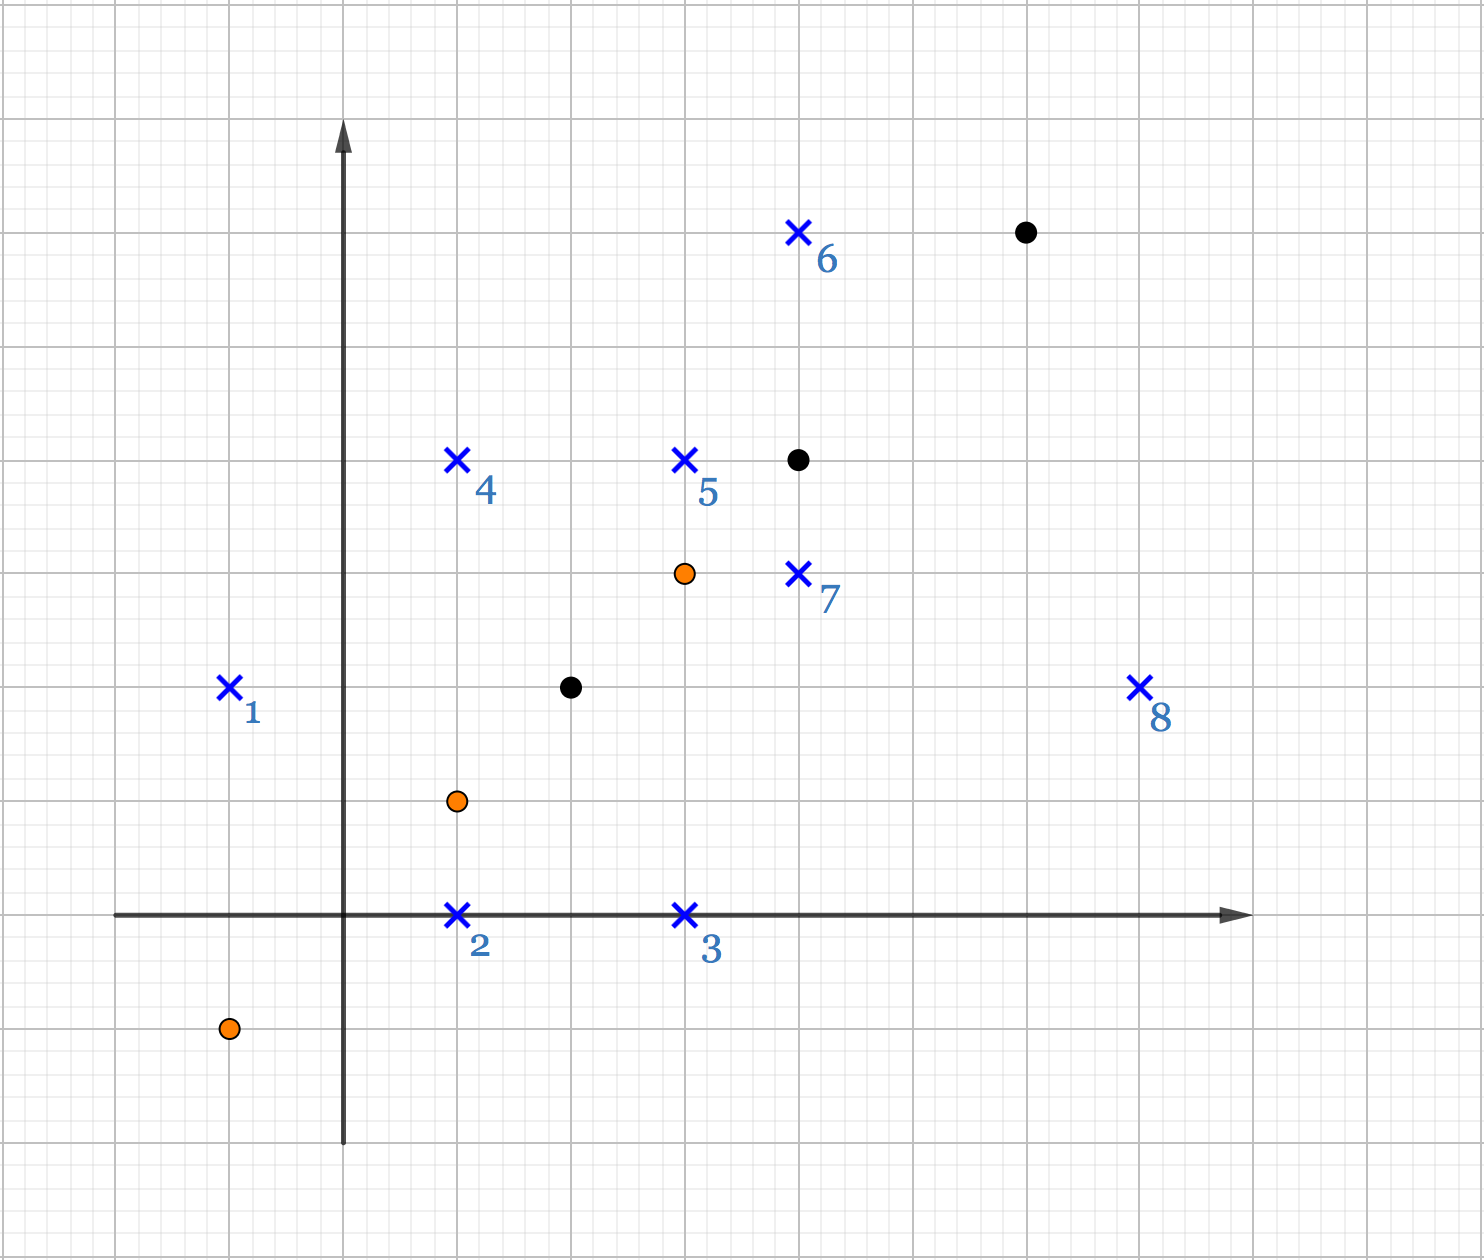
\includegraphics[scale=0.18]{2knn_1.png}
	\end{center} 
	
    Точка номер один явно будет в зоне влияния рыжих муравьёв. До ближайшего рыжего муравейника нужно пройти $\sqrt{5}$ метров, до ближайшего чёрного $3$ метра.  Точка два тоже рыжая. 
	
    По аналогии точки восемь и шесть оказываются чёрными. С оставшимися точками возникают проблемы. Например, от точки номер пять одинаковое расстояние как до чёрного, так и до рыжего муравейников. Она является спорной. Судя по всему, именно через неё пройдёт граница. Давайте попробуем нащупать побольше подобных пограничных точек. 
	
	Если точка принадлежит рыжим муравьям, будем помечать её рыжим крестом. Если чёрным, то чёрным. Если это спорная точка, то синим. 
	
	\begin{center}
	    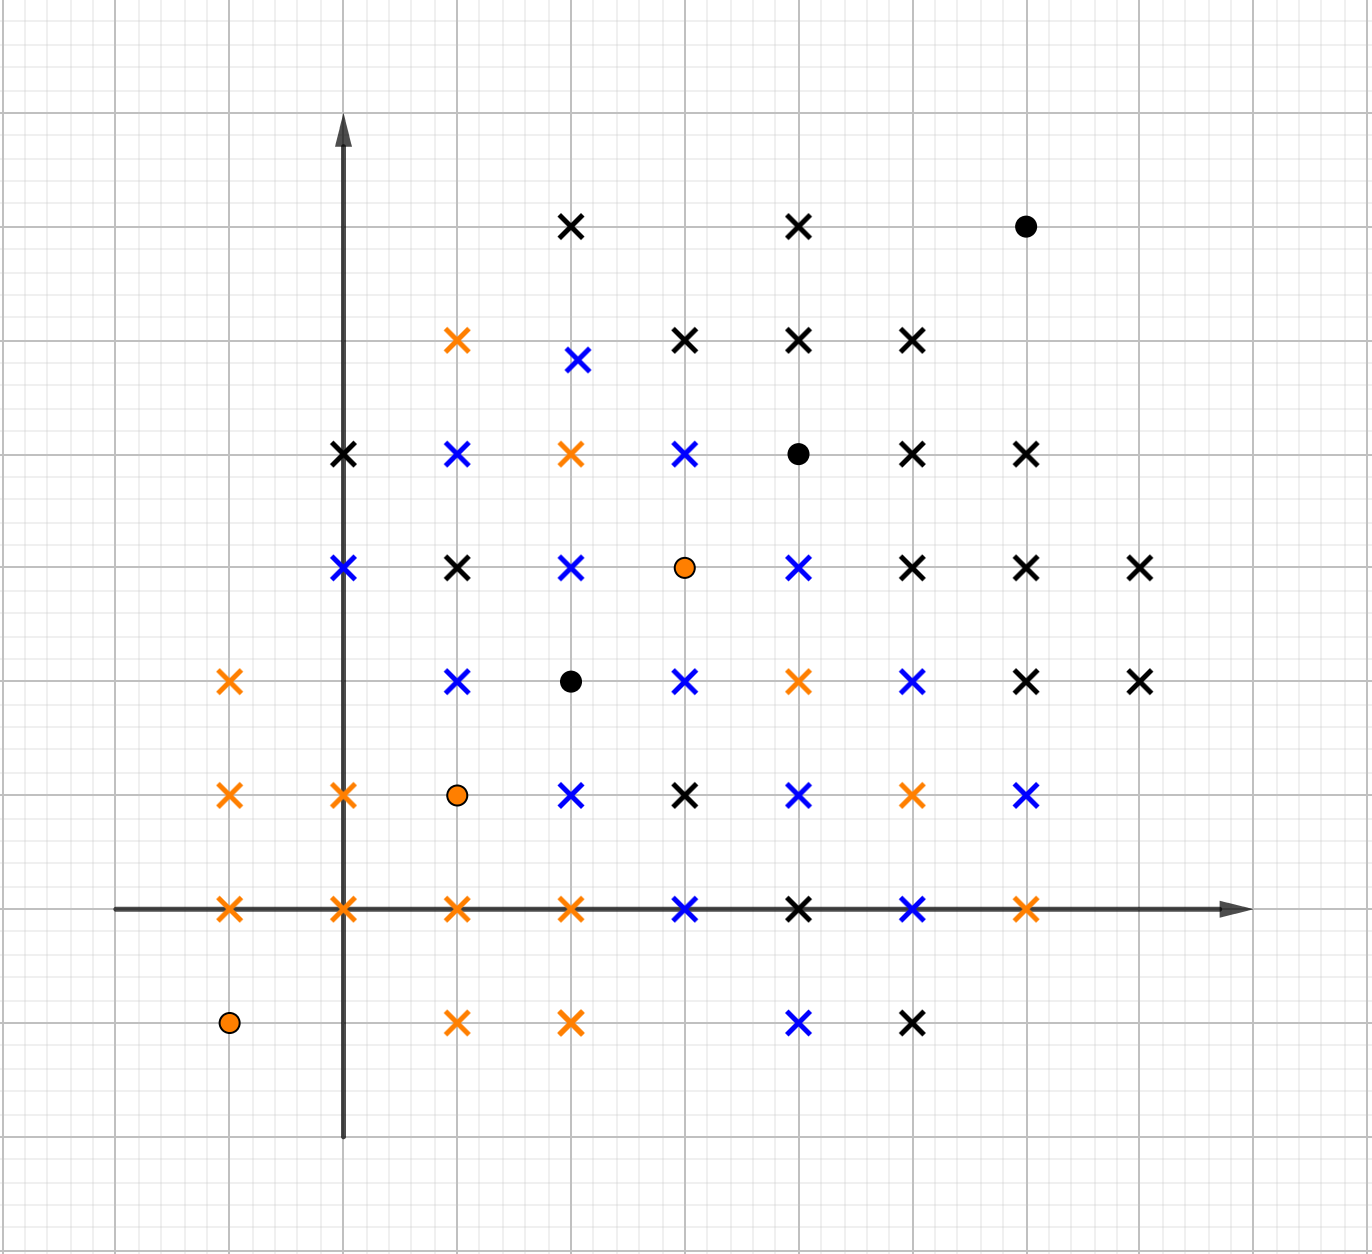
\includegraphics[scale=0.18]{2knn_2.png}
	\end{center} 
	
	Кажется, что мы нащупали границы, вдоль которых находятся спорные территории. Осталось только прочертить их.	
	
	\begin{center}
	    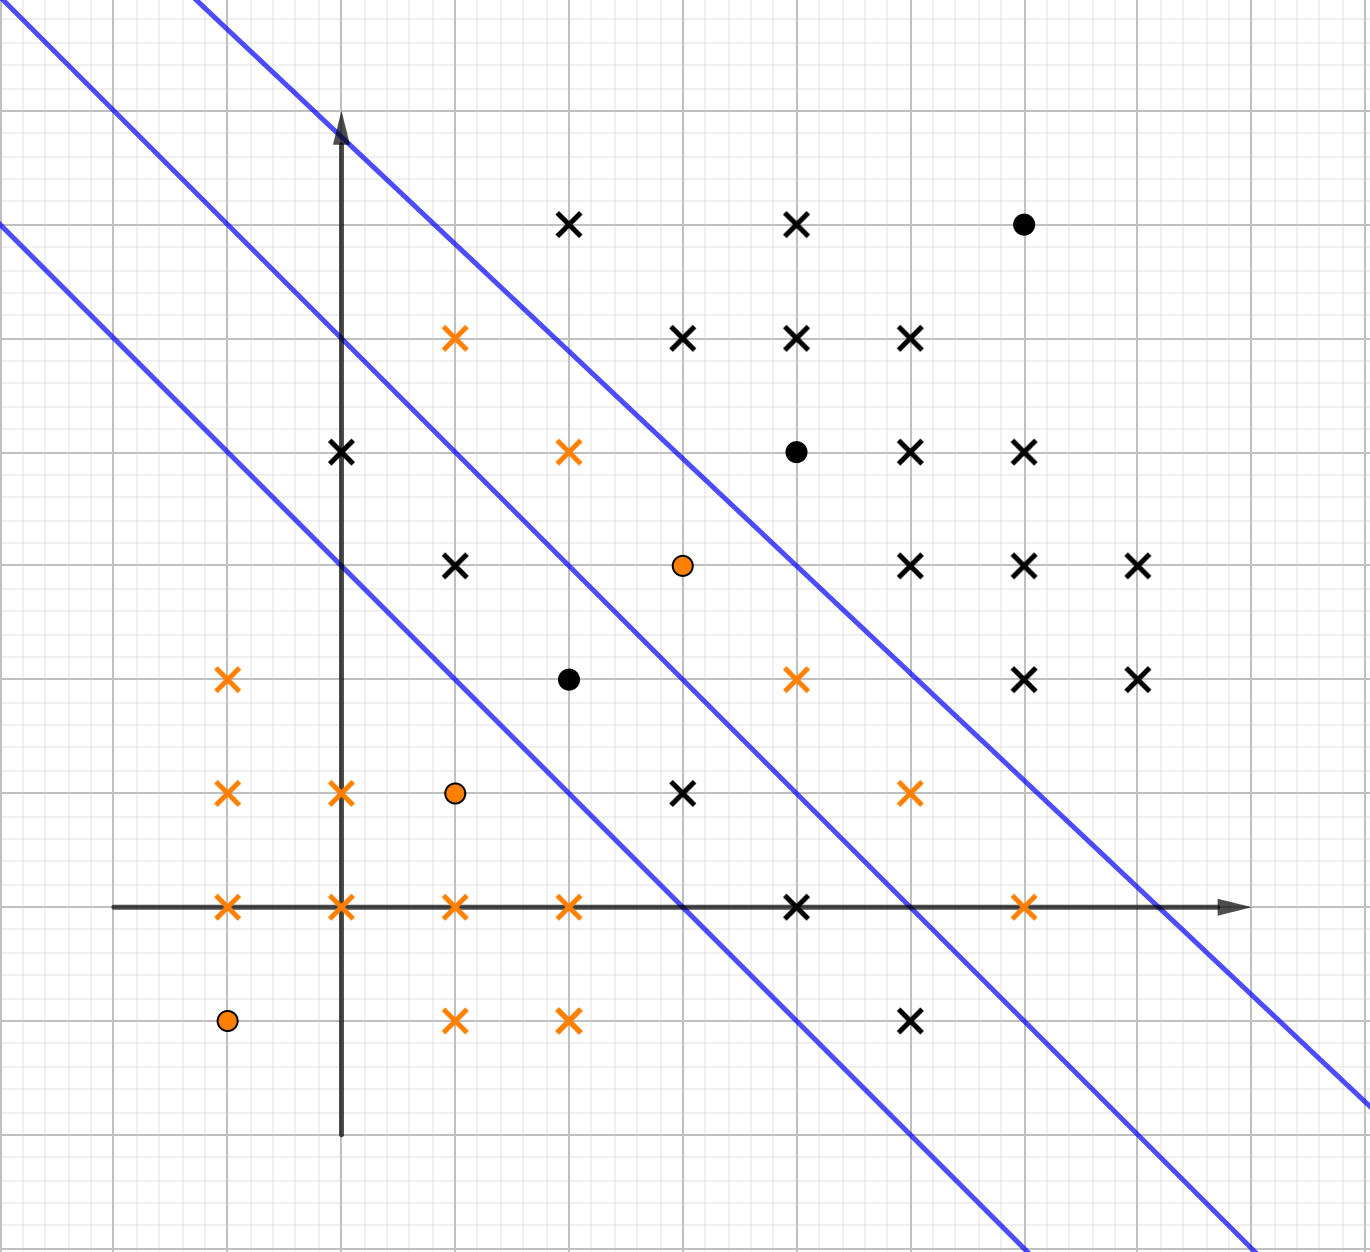
\includegraphics[scale=0.18]{2knn_3.png}
	\end{center} 
	
	\item[б)]  Теперь попробуем поделить плоскость на зоны влияния, используя метод трёх ближайших соседей. Посмотрим на самую первую картинку, где мы нанесли на плоскость рандомные точки, и попробуем порассуждать в чьей зоне влияния оказывается какая точка. 
	
	Для первой точки две из трёх ближайших --- рыжие. Она находится в рыжей зоне влияния. По аналогии происходит со второй и третьей точками.  Пятая, шестая, седьмая и восьмая точки оказываются в зоне влияния чёрных муравьёв и окрашиваются в чёрные цвета. Проблемы возникают только с четвёртой точкой. Ближайшие к ней две точки --- рыжая и чёрная. Решение надо принимать по третьему ближайшему соседу. Третью ближайшую точку найти не удаётся, так как рыжая и чёрная точка находятся от неё н одинаковых расстояниях. Выходит, что мы оказались на границе.
	
	\begin{center}
	    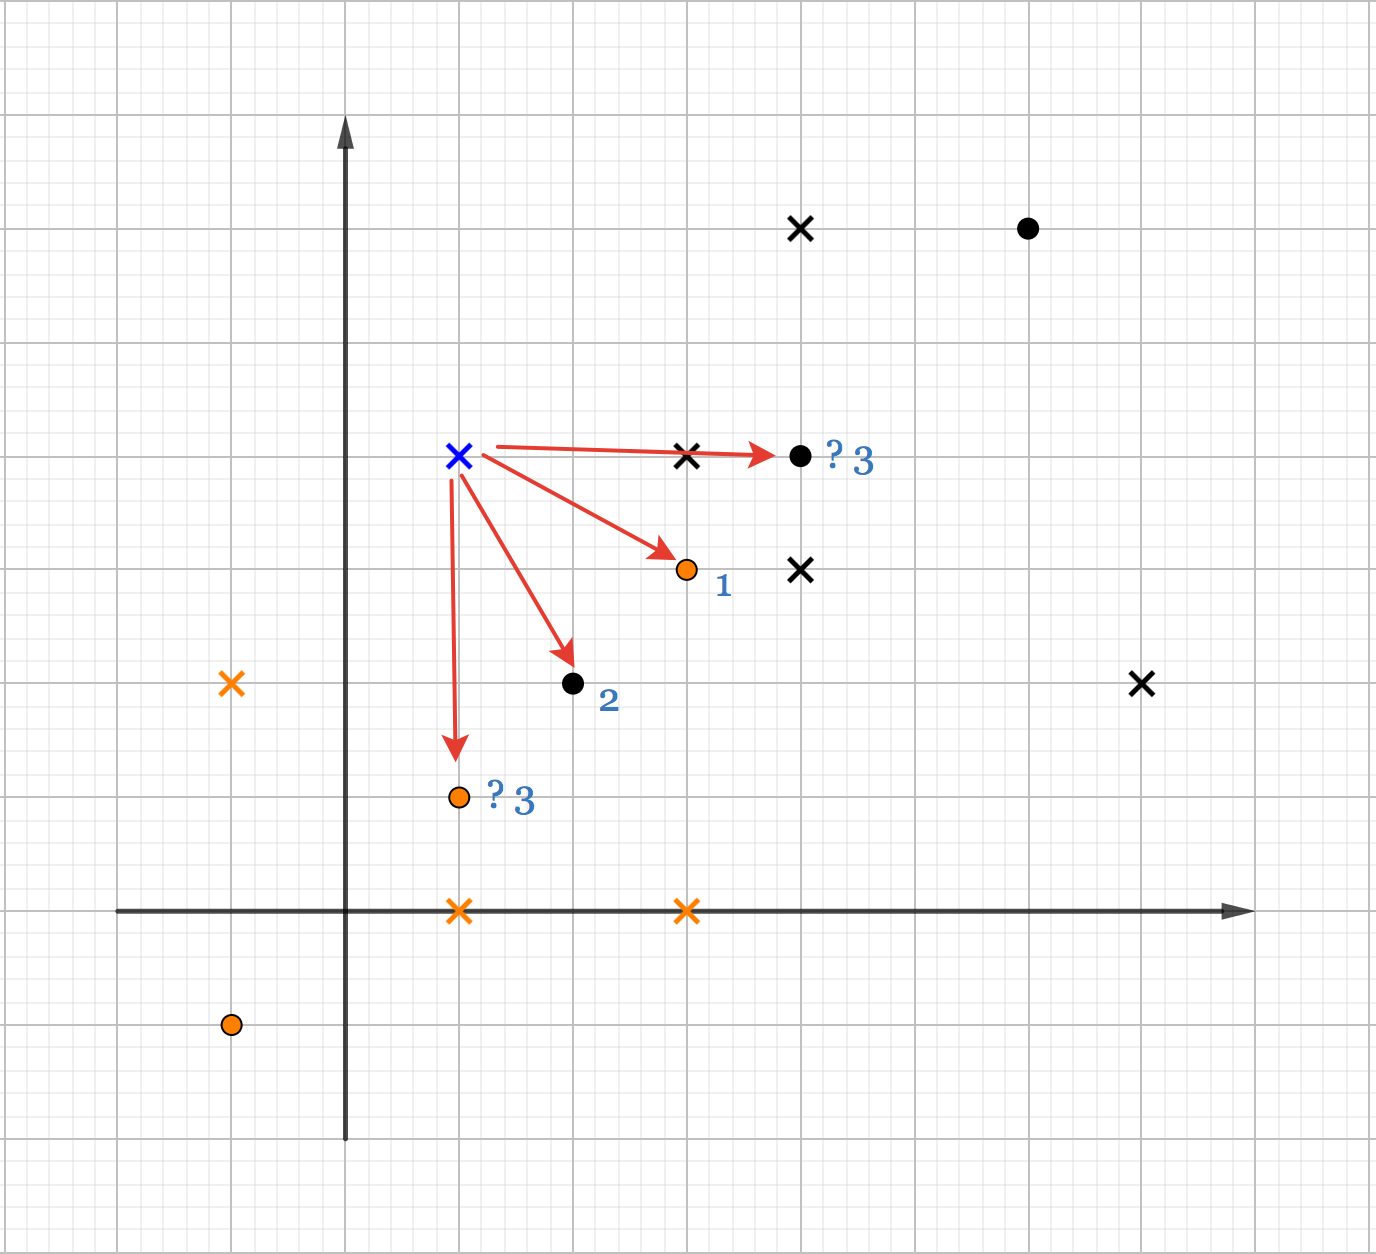
\includegraphics[scale=0.18]{2knn_4.png}
	\end{center} 

	Попробуем нащупать ещё пограничных точек и провести пограничную линию. 

	\begin{center}
	    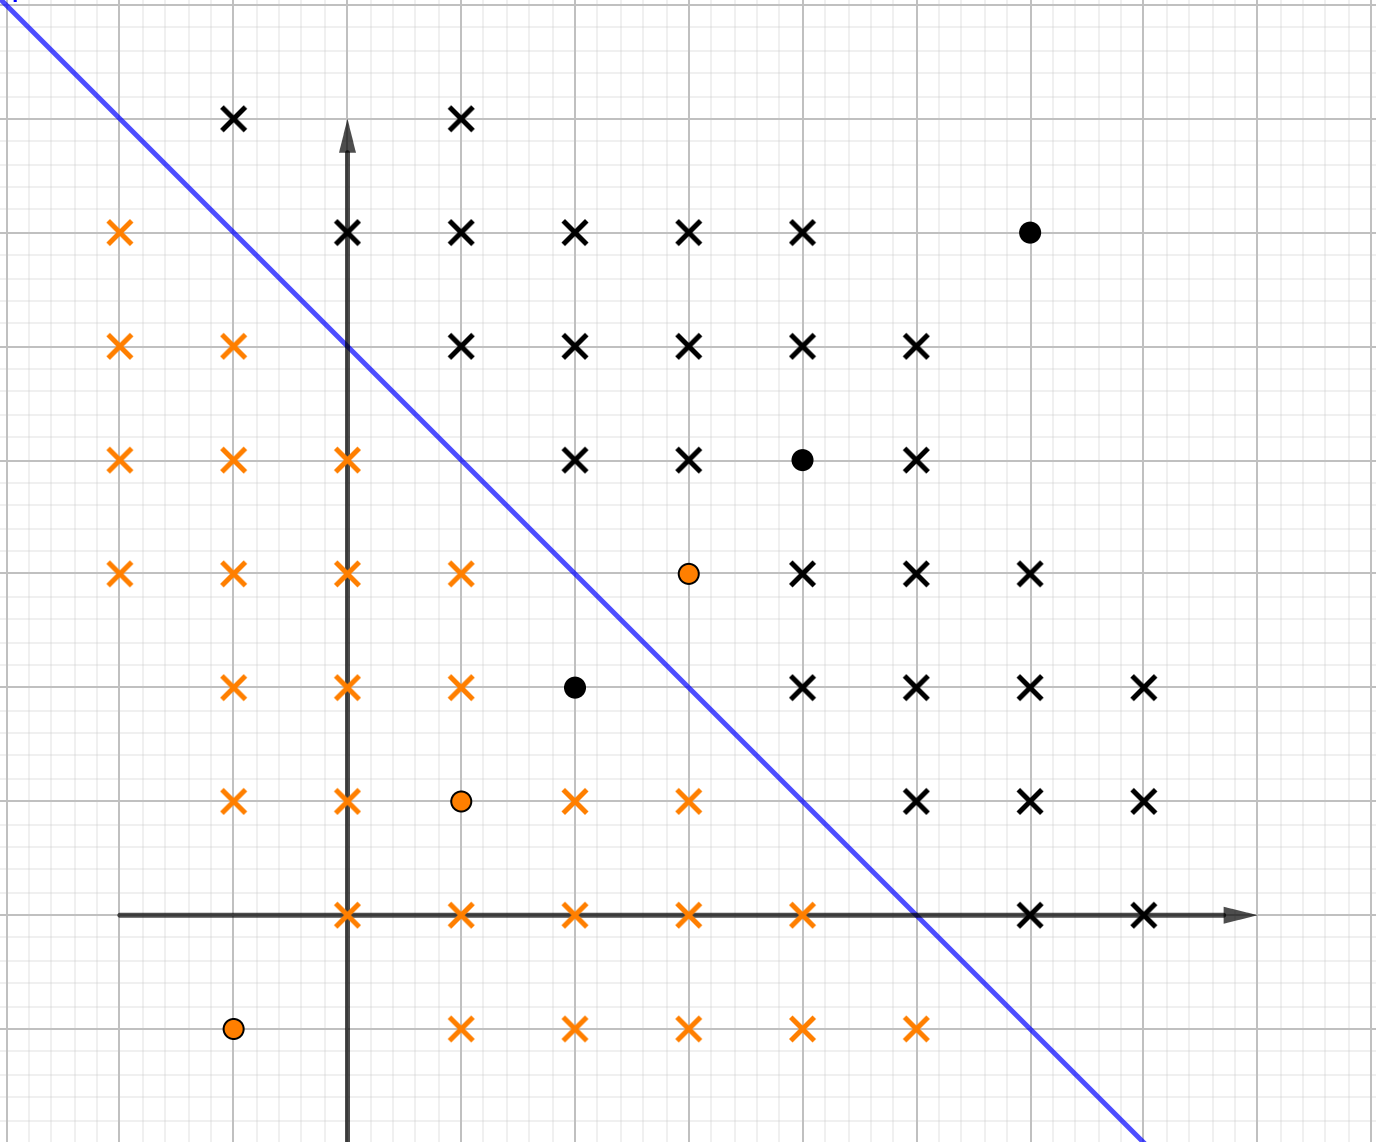
\includegraphics[scale=0.18]{2knn_5.png}
	\end{center} 	

	И это граница? У нас же есть ошибки!  Да, есть. Давайте вспомним упражнение про собачек, кошек, пиццу и бургеры с прошлого семинара. Когда мы решали его, мы поняли, что слишком детализированная граница между классами приводит к переобучению. 

	Порассуждаем в терминах джунглей. Есть поле, на нём селятся муравьи. Логично ли с их стороны селиться полосками? Конечно же нет. Намного логичнее было бы, что по историческим причинам на одной стороне поля живут рыжие муравьи, на второй чёрные. У нас в выборке оказалось несколько примеров муравейников. И по ним мы попытались нащупать границу для зон влияния. На границе вполне может происходить такое, что муравьи проникают на территорию друг-друга. 

	Проводя излишние полосы, мы переходим от выуживания реальных закономерностей, существующих в джунглях, к излишнему фрагментированию обучающей выборки, то есть переобучаемся под её особенности. Практически все алгоритмы машинного обучения страдают этим грехом. Нам надо будет как следует бить их за переобучение и исправлять.

	\item[в)]  Давайте убедимся в том, что алгоритм трёх ближайших соседей, проводящий одну разграничительную линию между муравьями, работает лучше, чем алгоритм одного ближайшего соседа. Для этого воспользуемся стратегией кросс-валидации. 

	Кросс-валидация состоит в следующем: давайте будем закрывать по очереди разные части выборки ладошкой. На оставшейся выборке будем обучать модель, а на скрытой проверять её качество. Будем делать так много раз и посмотрим на итоговое качество. 
	
	\begin{minipage}[t]{0.45\textwidth}
	    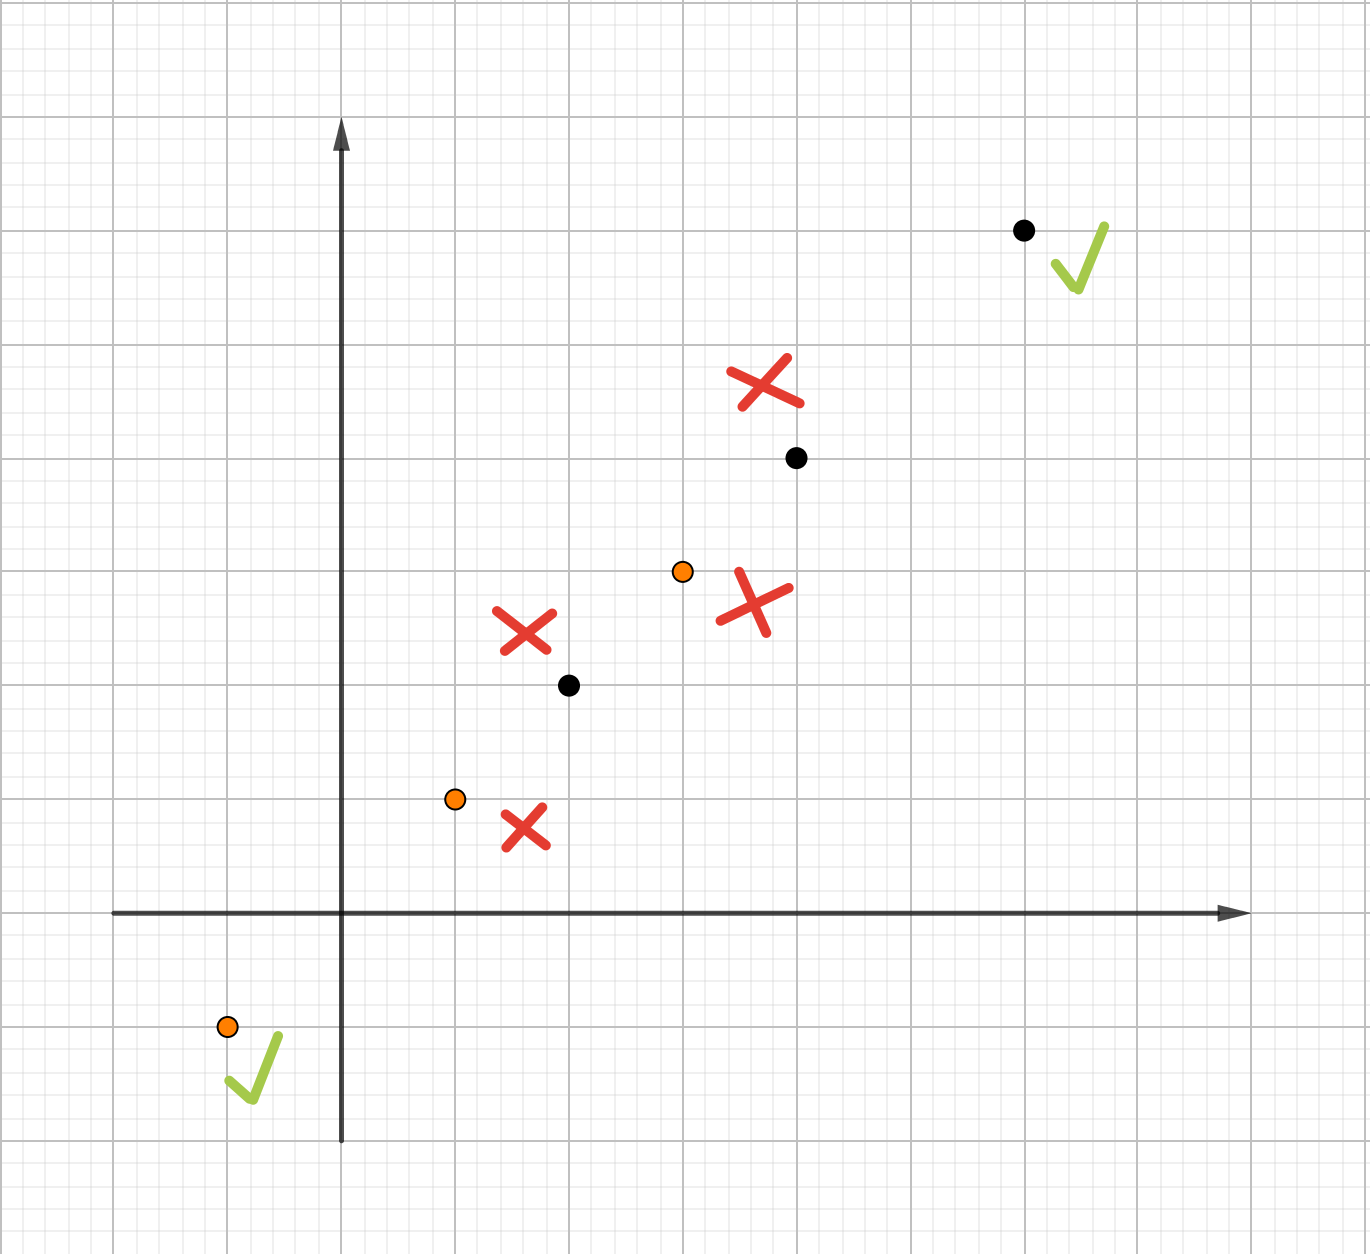
\includegraphics[scale=0.15]{2knn_6.png}
	\end{minipage}
	\hfill
	\begin{minipage}[t]{0.45\textwidth}
	    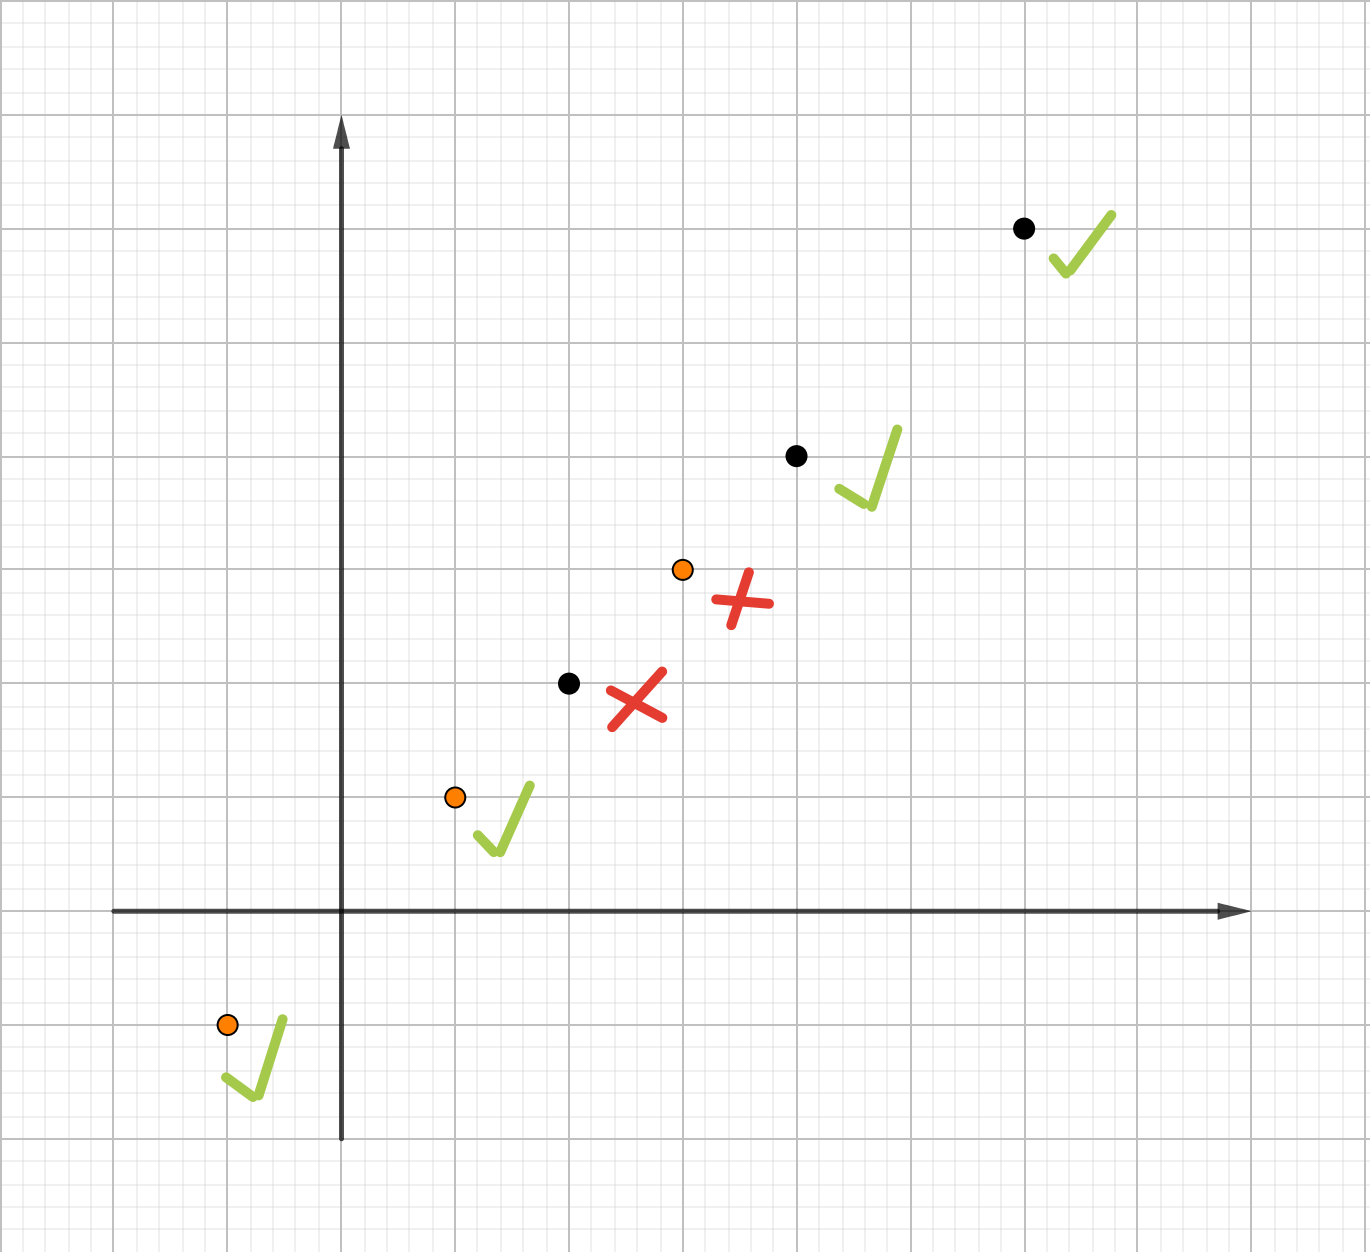
\includegraphics[scale=0.15]{2knn_7.png}
	\end{minipage}
	
	Закрываем ладошкой самую нижнюю точку. По оставшимся четырём расчерчиваем границы. Мы по методу одного ближайшего соседа относим эту точку к рыжим муравьям. Это оказывается правильным решением. Угадали.

	Закроем ладошкой вторую снизу точку. Расчертим границы. Она окажется ближе всего к чёрным муравьям. Но на самом деле она рыжая. Ошибка... Также проделаем с остальными точками. В итоге получится, что мы совершаем целых $4$ ошибки. По аналогии сделаем с методом трёх ближайших соседей и получим всего лишь $2$ ошибки. 

	Чувствуете? Мы ошибаемся из-за излишней детализации, которую нам навязывает метод одного ближайшего соседа. Кросс-валидация позволяет это отследить. А что, если взять $5$ ближайших соседей? Тогда мы ошибёмся абсолютно в каждой точке. Попробуйте проделать это. 

	На самом деле $k$ это \indef{гиперпараметр} метода ближайших соседей. Мы можем подобрать его оптимальным образом с помощью кросс-валидации. В данном примере оптимально будет выбрать $k=3$. 
	
	В этом упражнении мы использовали для оптимизации алгоритма метрику accuracy. Понятное дело, что можно пытаться использовать и любую другую метрику с прошлого семинара. 
	\end{enumerate}
\end{solution}

\begin{problem}{(древо для классификации)}
У Маши есть инстаграмчик. На неё подписана целая куча парней. Недавно Дима поставил ей $10$ лайков. Тогда Маша схватила ромашку и начала гадать. Она нагадала, что Дима плюнет в неё. То же самое она сделала с другими парнями. 

Результат гадания --- переменная $y_i$, количество лайков у фотки --- переменная $x_i$. 

\begin{center}
	\begin{tabular}{cc}
		$y_i$ & $x_i$ \\
		\hline
		плюнет & $10$ \\
		поцелует & $11$ \\
		поцелует & $12$ \\
		к сердцу прижмёт & $13$ \\
		к сердцу прижмёт & $14$ \\
	\end{tabular}
\end{center}

Сегодня в Машином инстаграмме Джонни Деп поставил $15$ лайков. Маше очень хочется понадать что же с ней сделает Джонни Деп, но у неё кончились ромашки. Поэтому она решила обучить классификационное дерево, которое поможет ей спрогнозировать $y_i$ по $x_i$.

Дерево строится до идеальной классификации. Критерий деления узла на два --- минимизация числа допущенных ошибок\footnote{На самом деле на практике так не делают. Обычно для разбиения узла при строительстве классификационных деревьев используют энтропию. О том, что это такое, можно погуглить.}.  Правило прогнозирования в каждой вершине: в качестве прогноза выдаем тот класс, представителей которого в вершине больше.
\end{problem}

\begin{solution}
Мы должны обучить дерево, которое будет по переменной $x$, число лайков от парня, прогнозировать переменную $y$, состояние отношений Маши.  Обычно деревья учат по-жадному. Будем смотреть, какое разбиение по переменной $x$ сильнее всего уменьшает ошибку, и выбирать его. 
	
Ошибку мы договорились считать как долю неверных ответов. Обычно на практике при разбиении вершины на две используют не такой критерий, но мы для простоты используем его.

Будем перебирать все возможные пороги и смотреть что получится.
	
При делении вершины на две между $10$ и $11$ лайками, слева у нас окажется плюнет. Именно его мы и будем там прогнозировать. Справа окажется два поцелует и два к сердцу прижмёт. Надо спрогнозировать в этой вершине класс, представителей которого тут большинство, чтобы сделать поменьше ошибок. Так как у нас оба класса представлены в одинаковом объёме, неважно что мы спрогнозируем. В любом случае получим две ошибки. 
	
При дроблении вершины на две между $11$ и $12$ лайками, слева оказывается плюнет и поцелует. Одна ошибка. Справа оказывается два к сердцу прижмёт и одно поцелует. Спрогнозируем к сердцу прижмёт, так как их большинство, и получи одну ошибку. В сумме у нас две ошибки. 
	
\begin{center}
    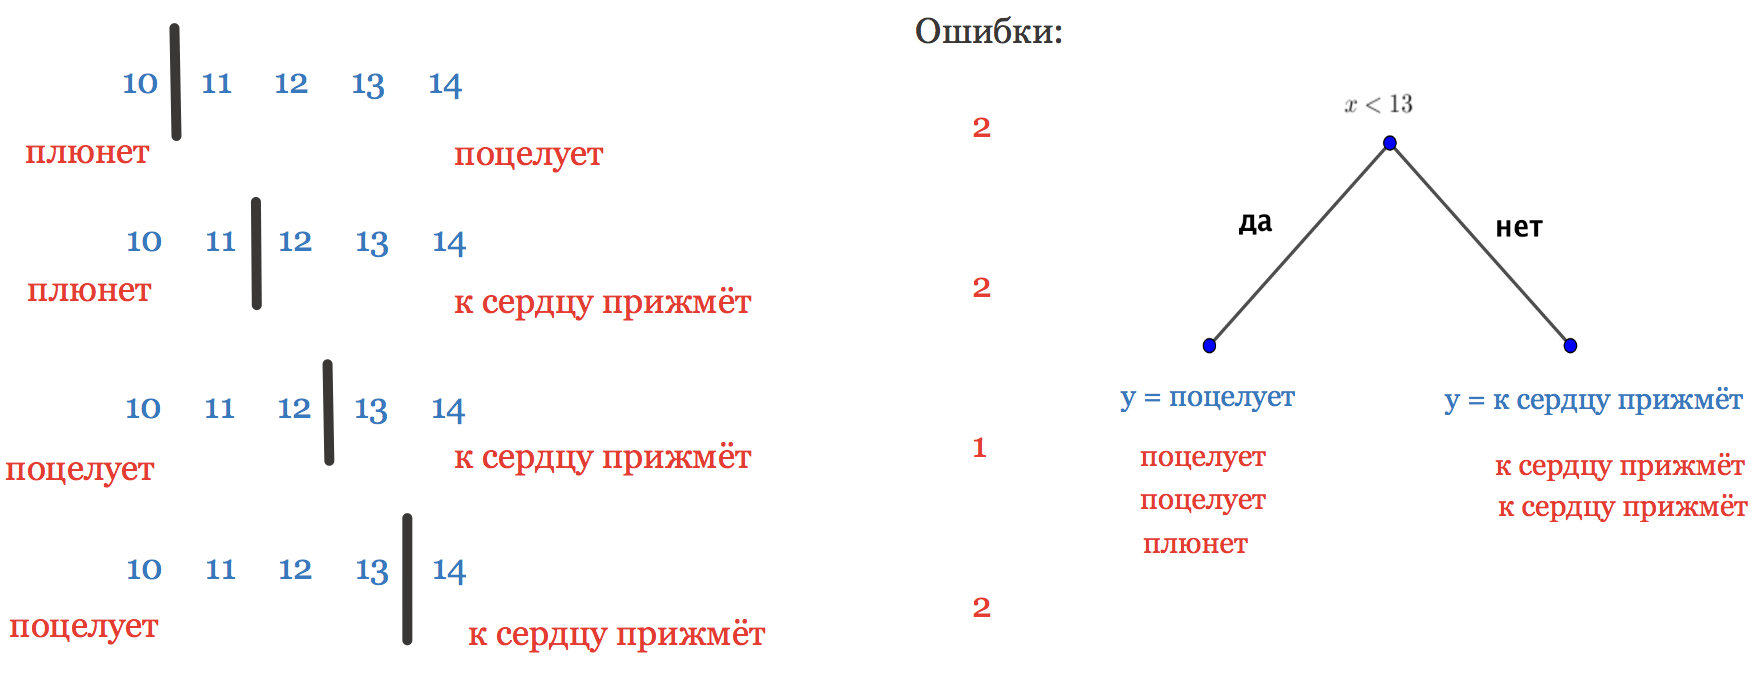
\includegraphics[scale=0.28]{class_tree_1.png}
\end{center} 	
	
Рассуждая аналогичном образом приходим к выводу, что самое классное разбиение между $12$ и $13$. При нём мы совершаем только одну ошибку.  В дереве, мы будем задавать вопрос: <<А количество лайков меньше $13$?>> Если да, будем идти налево и прогнозировать, что нас поцелуют. Если нет, будем идти направо и прогнозировать, что нас прижмут к сердцу. 
	
Справа в листе дерева у нас оказались объекты одного класса. Слева в листе дерева соодержутся объекты разных классов. Можно сделать ещё одно разбиение. 
	
\begin{center}
	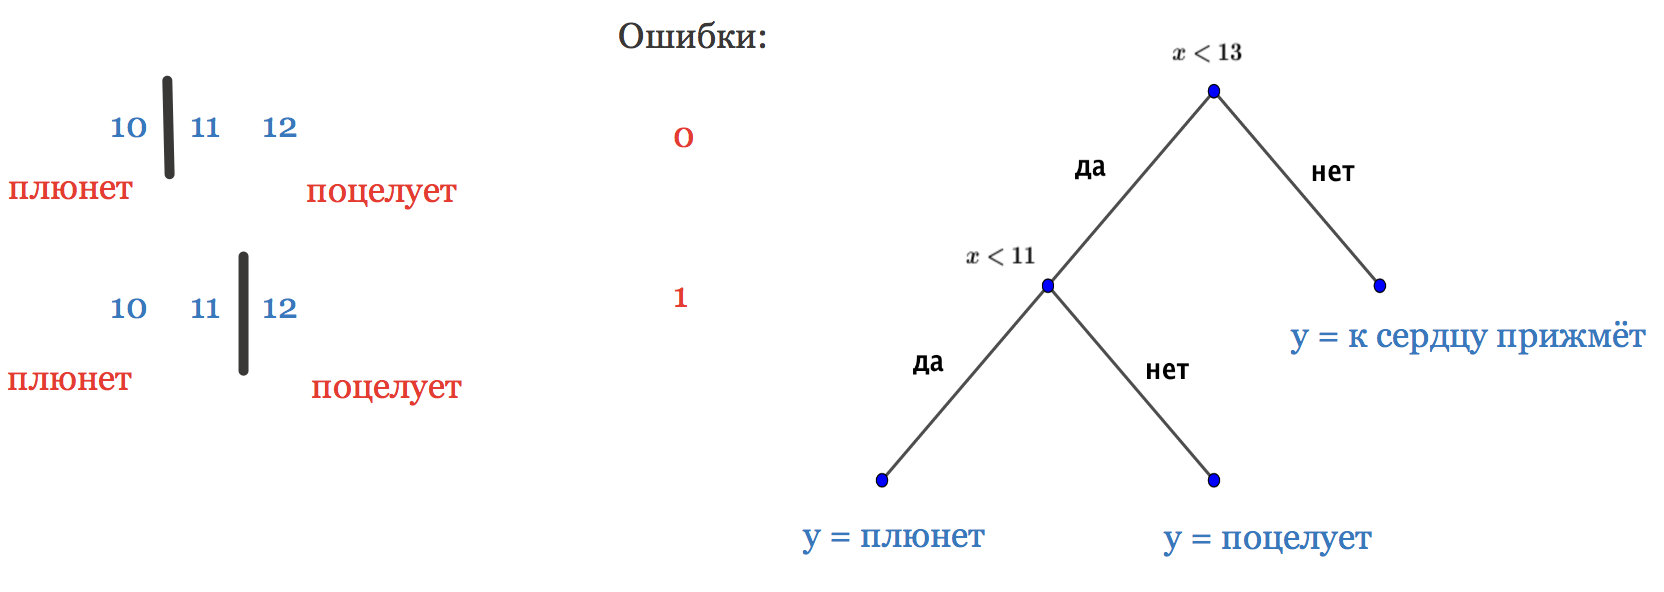
\includegraphics[scale=0.28]{class_tree_2.png}
\end{center} 	

В итоге в нашем дереве окажется три листа, в каждом из которых мы будем делать прогноз. Обратите внимание, что дерево запомнило выборку.  Деревья постоянно так делают. В этом их сушественный минус. Чтобы победить его, деревья стригут. Либо используют как части более сложных моделей. Например, как часть случайного леса. 
	
Джонни поставил Маше $15$ лайков. Что же ожидает их отношения? Начинаем идти по решающему дереву, чтобы сделать прогноз. Число лайков меньше $13$? Нет. Идём направо. Кажется, Машу прижмут к сердцу. Это наш прогноз.  	
\end{solution}

\begin{problem}{(ещё деревья)}
Ниже изображены разделяющие поверхности для задачи бинарной классификации, соответствующие решающим деревьям разной глубины. Какое из изображений соответствует наиболее глубокому дереву? Какой примерной глубине дерева соответствует каждая из картинок? 

\begin{center}
	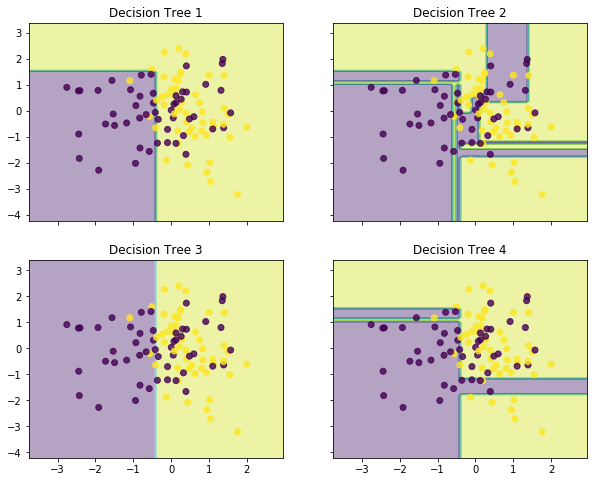
\includegraphics[scale=0.6]{trees.png}
\end{center}
\end{problem}

\begin{solution}
Чем глубже дерево, тем сильнее оно фрагментирует нашу выборку, и тем сильнее оно выделяет в ней самые микроскопические кусочки.  Сильнее всего выборка фрагментирована на верхней правой картинке, значит это разбиение плоскости на части соответствует самому глубокому дереву. 

На третьей картинке плоскость дробиться на части один раз. Значит в дереве есть один сплит. Его глубина равна единице. На первой картинке появляется ещё одно дополнительное разбиение по оси $y$, глубина дерева увеличивается до двух. 

На картинке номер $4$ мы делаем два дополнительных разбиения правой части и два левой. Глубина дерева уже не менее трёх. На второй картинке всё становится ещё глубже. 
\end{solution}

\section*{Ещё задачи} 

Тут лежит ещё несколько задач для самостоятельного решения. Возможно, похожие будут в самостоятельной работе... 

\begin{problem}{}
На плоскости расположены колонии рыжих и чёрных муравьёв. Рыжих колоний три и они имеют координаты $(-1, 1)$, $(1, -1)$ и $(1, 1)$. Чёрных колоний одна и она имеет координаты $(0, 0)$.

\begin{enumerate}
\item[а)] Поделите плоскость на «зоны влияния» рыжих и чёрных используя метод одного и трёх ближайших соседей.

\item[б)] С помощью кросс-валидации с выкидыванием отдельных наблюдений выберите оптимальное число соседей $k$ перебрав $k \in \{1, 3 \}$. Целевой функцией является количество несовпадающих прогнозов.
\end{enumerate}
\end{problem}

\begin{problem}{}
Объясните мемас: 

\begin{center}
	
\includegraphics[scale=0.3]{memes2.jpg}
\end{center}
\end{problem}

\begin{problem}{}
Пятачок собрал данные о визитах Винни-Пуха в гости к Кролику. Здесь $x_i$ --- количество съеденного мёда в горшках, а $y_i$  --- бинарная переменная, отражающая застревание Винни-Пуха при входе 

\begin{center}
	\begin{tabular}{c|c}
		$y_i$ & $x_i$ \\
		\hline
		0  & 1 \\
		1 & 4\\
		1 & 2\\
		0 & 3 \\
		1 & 3 \\
		0 & 1
	\end{tabular}
\end{center}

\begin{enumerate}
	\item[а)] Пятачок собирается оценить дерево по всей выборке.  Помогите очень маленькому существу сделать это. 
	\item[б)] Пятачок узнал у Иа-Иа, что оказывается выборку надо делить на тренировочную и тестовую Поэтому он отложил последние два наблюдения для теста. Оцените дерево по первым четырём наблюдениям и проверьте его работоспособность по последним двум. 
	\item[в)]  Пятачок поговорил с Совой и узнал, что деревья часто переобучаются. Она рассказала ему, что над деревьями надо строить ансамбли. Например, случайный лес. Пятачок решил построить лес из трёх деревьев. Первое дерево он строит на наблюдениях с первого по третье, второе на наблюдениях со второго по четвёртое.  Третье дерево на наблюдениях $1,2,4$. Помогите пяточку построить лес и оценить качество его работы на тестовой выборке. 
\end{enumerate}
\end{problem}

\begin{solution}
\begin{enumerate}
	\item[а)]  Бедный малютка Пяточок! Он даже не понимал, на какие муки он себя обрекает, когда собирался строить свою модель для прогнозирования того, что произойдёт с Винни! Как же хорошо, что мы оказались рядом и подставили маленькому существу своё большое дружеское плечо.  Для начала построим дерево сразу на всей выборке. 
	
	\begin{center}
	    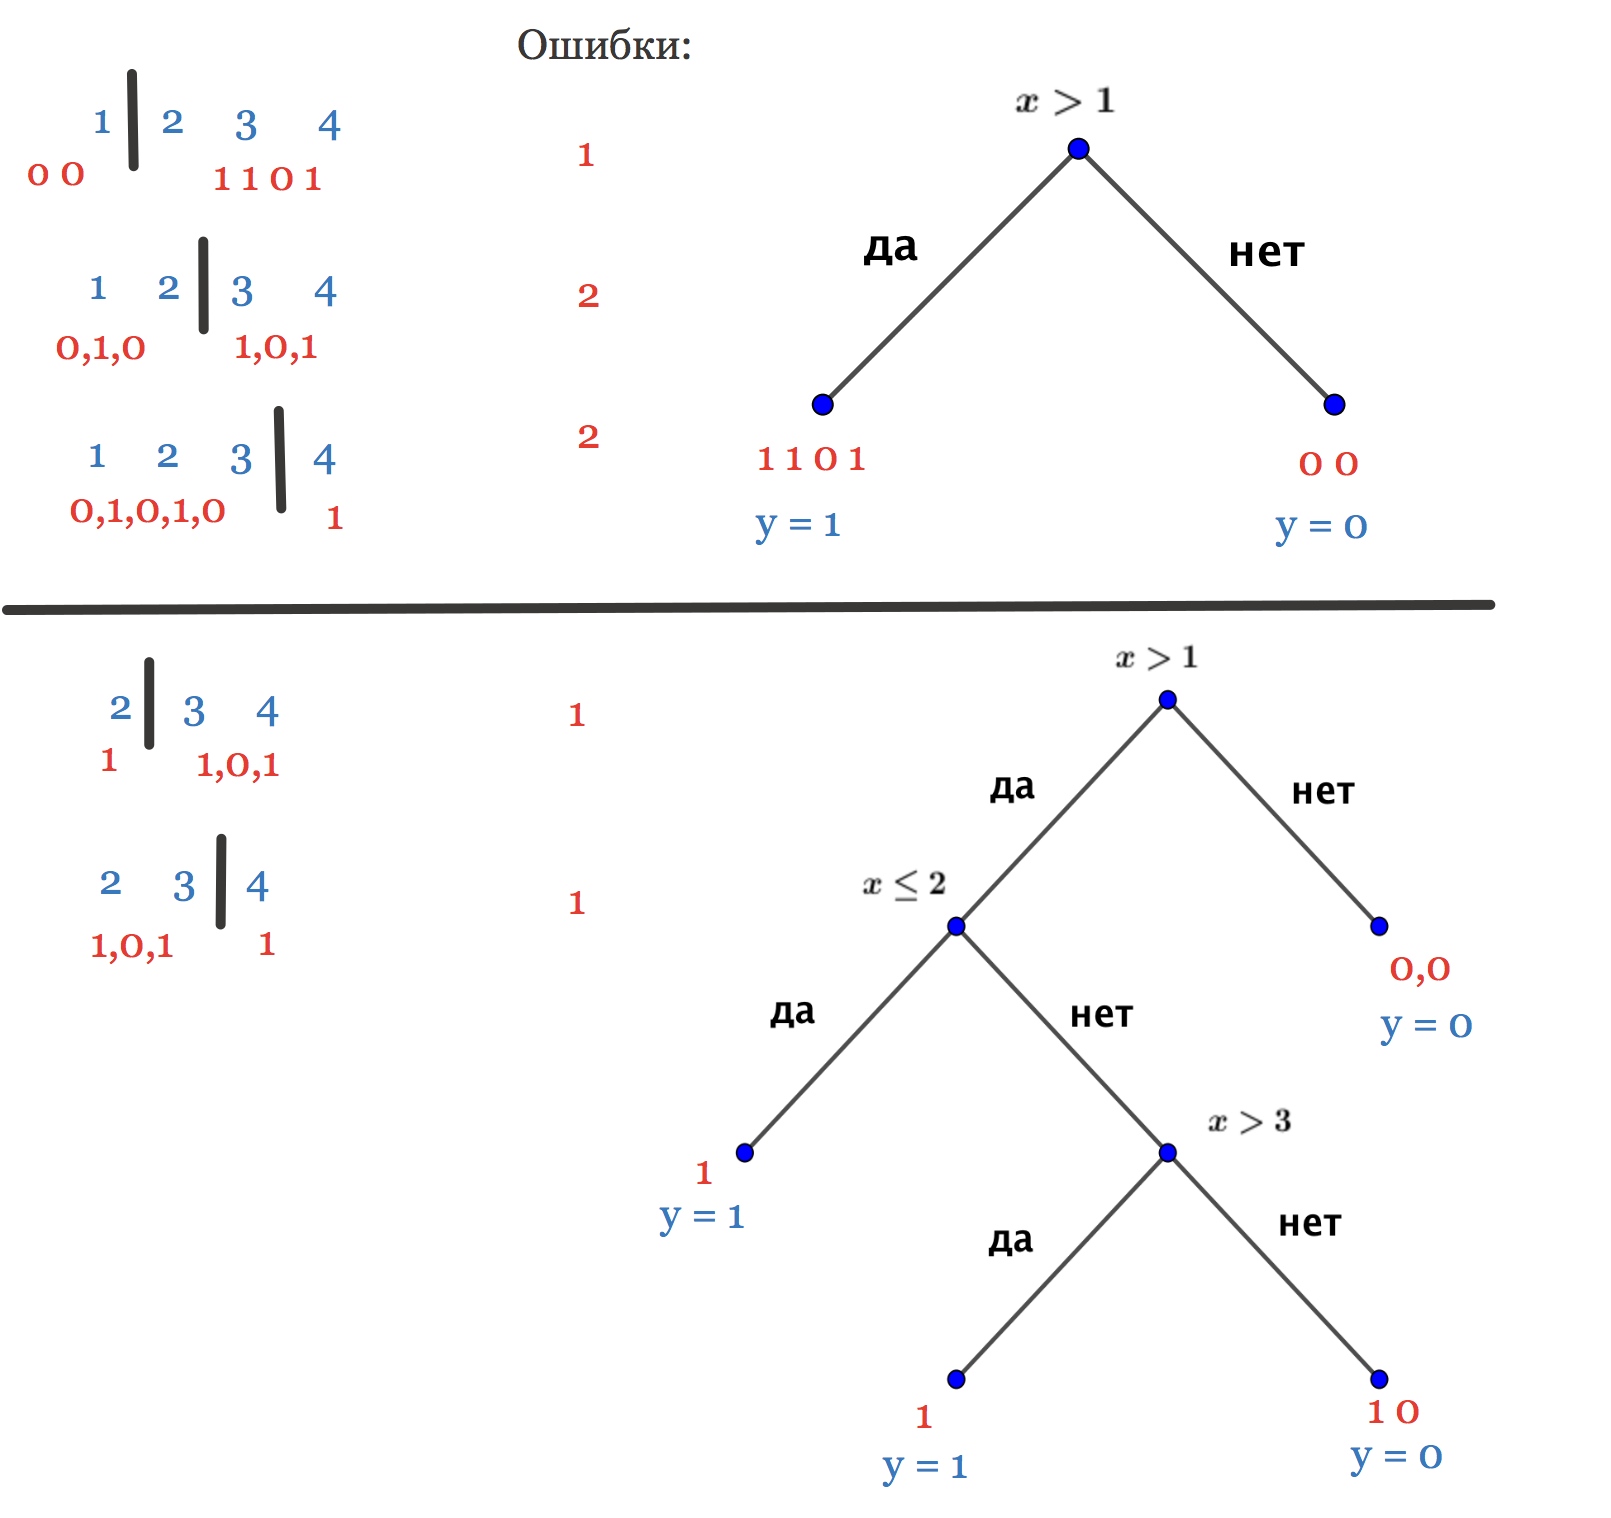
\includegraphics[scale=0.28]{class_tree_6.png}
	\end{center} 	

	Обратите внимание, что это дерево ошибается из-за того, что при  $x=3$ у нас есть как факт застревания медведя в норе, так и факт его прохождения сквозь нору. Когда мы оказываемся в вершине, где одинаковое число нулей и единиц, нам придется принимать решение случайно. Компьютер поступает именно так. На больших выборках это случаентся довольно редко. 

	\item[б)]  Когда мы строим дерево на первых четырёх наблюдениях, первое разбиение можно сделать либо по единице, либо по четвёрке. В обеих ситуациях совершается одна ошибка. Для удобства выберем первый случай. Дальше снова неважно где делать разбиение. Сделаем его в двойке. В итоге получим дерево из пункта а). На тестовой выборке дерево делает одну ошибку при $x=3$.
	
	\item[в)]   Лес, который должен получиться в ходе обучения, изображён на кратинке: 
	
	
	\begin{center}
		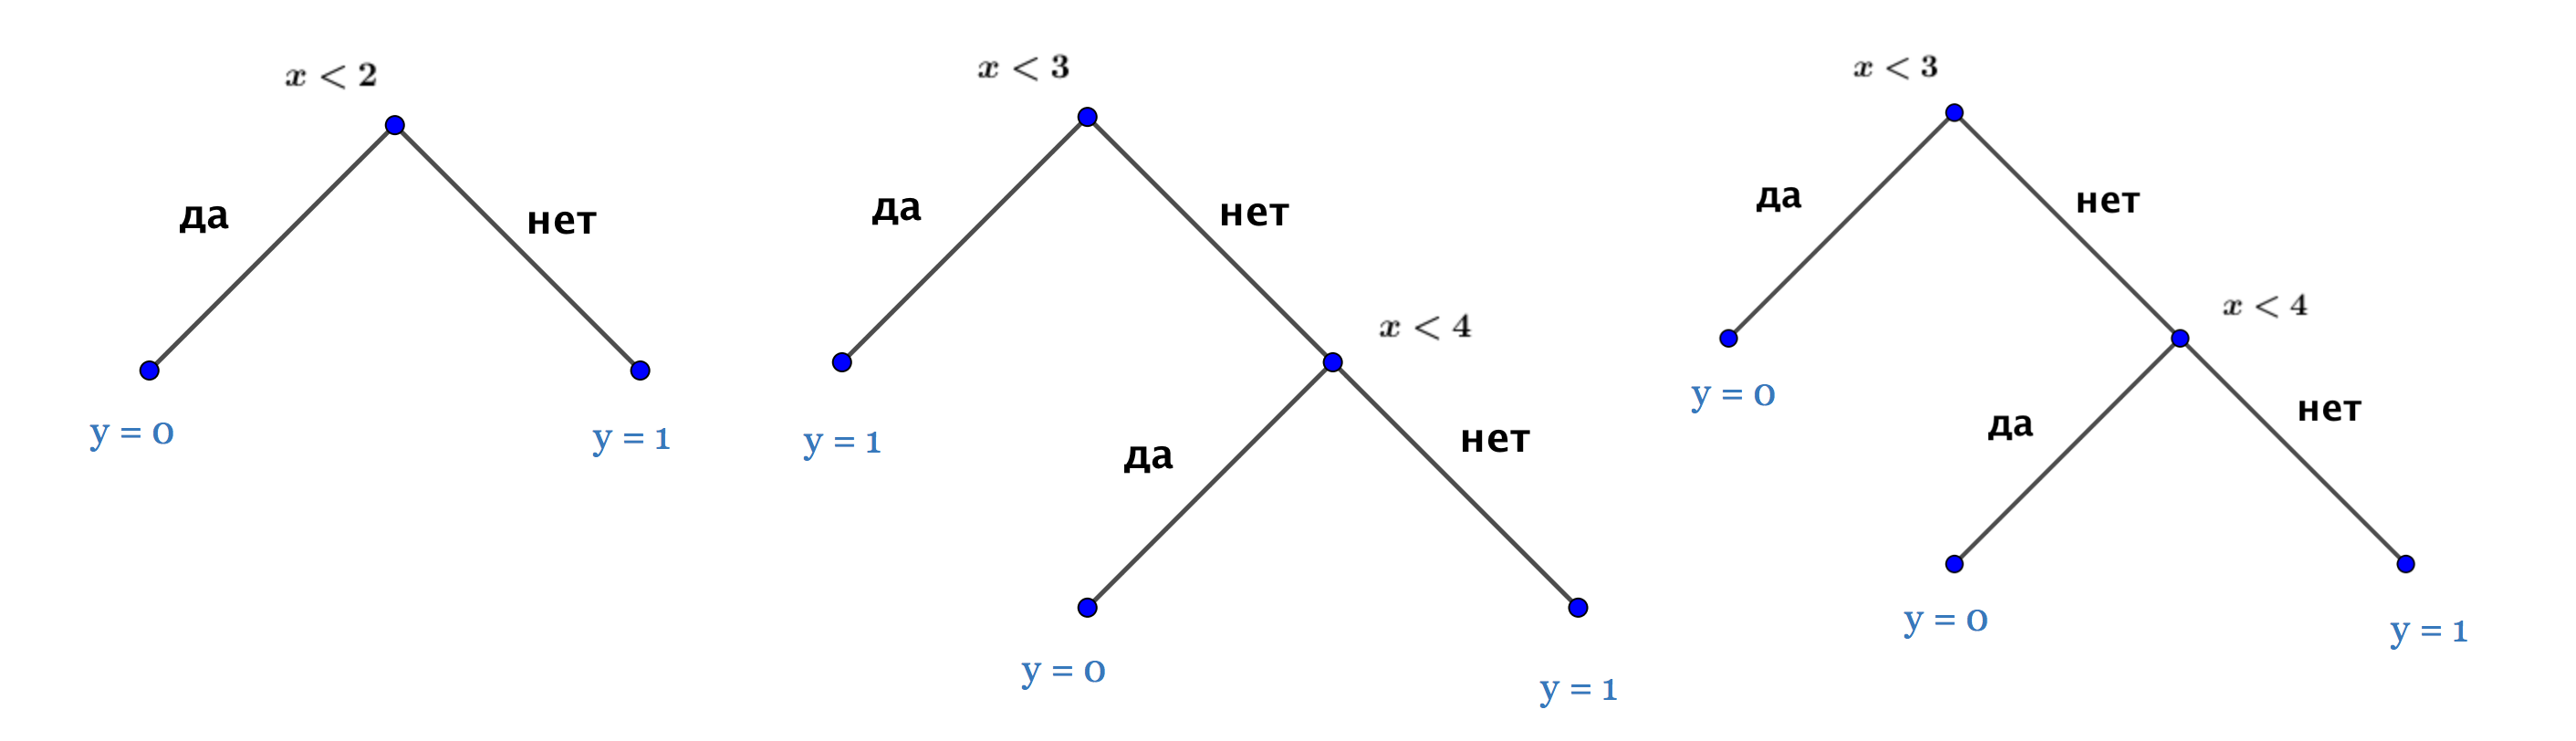
\includegraphics[scale=0.17]{forest.png}
	\end{center} 	
	
	Для $x=3$ первое дерево прогнозирует $1$, второе $0$, третье $0$. Большая часть леса говорит, что прогнозом будет $0$. Верим в торжество демократии и берём его в качестве итогового прогноза. Допускаем ошибку\footnote{Демократия не идеальна, но это лучшее, что придумало человечество}. Для $x=1$ первое и третье деревья прогнозируют $0$, второе $1$, берём ноль и не ошибаемся. Прогноз по лесу построен.
	
	На практике случайный лес показывает себя как очень мощный алгоритм. Не стесняйтесь использовать его. 
\end{enumerate}
\end{solution}

\begin{problem}{}
По данной диаграмме рассеяния постройте классификационное дерево для зависимой переменной $y$:

\begin{center}
	\begin{tikzpicture}[scale = 0.015]
	% Created by tikzDevice version 0.10.1 on 2017-03-21 20:23:18
% !TEX encoding = UTF-8 Unicode
\definecolor{fillColor}{RGB}{255,255,255}
\path[use as bounding box,fill=fillColor,fill opacity=0.00] (0,0) rectangle (505.89,505.89);
\begin{scope}
\path[clip] (  0.00,  0.00) rectangle (505.89,505.89);
\definecolor{drawColor}{RGB}{255,255,255}
\definecolor{fillColor}{RGB}{255,255,255}

\path[draw=drawColor,line width= 0.6pt,line join=round,line cap=round,fill=fillColor] (  0.00,  0.00) rectangle (505.89,505.89);
\end{scope}
\begin{scope}
\path[clip] ( 38.98, 29.52) rectangle (448.08,500.39);
\definecolor{fillColor}{RGB}{255,255,255}

\path[fill=fillColor] ( 38.98, 29.52) rectangle (448.08,500.39);
\definecolor{drawColor}{gray}{0.92}

\path[draw=drawColor,line width= 0.3pt,line join=round] ( 38.98,104.50) --
	(448.08,104.50);

\path[draw=drawColor,line width= 0.3pt,line join=round] ( 38.98,211.99) --
	(448.08,211.99);

\path[draw=drawColor,line width= 0.3pt,line join=round] ( 38.98,319.48) --
	(448.08,319.48);

\path[draw=drawColor,line width= 0.3pt,line join=round] ( 38.98,426.97) --
	(448.08,426.97);

\path[draw=drawColor,line width= 0.3pt,line join=round] (104.14, 29.52) --
	(104.14,500.39);

\path[draw=drawColor,line width= 0.3pt,line join=round] (197.47, 29.52) --
	(197.47,500.39);

\path[draw=drawColor,line width= 0.3pt,line join=round] (290.79, 29.52) --
	(290.79,500.39);

\path[draw=drawColor,line width= 0.3pt,line join=round] (384.11, 29.52) --
	(384.11,500.39);

\path[draw=drawColor,line width= 0.6pt,line join=round] ( 38.98, 50.75) --
	(448.08, 50.75);

\path[draw=drawColor,line width= 0.6pt,line join=round] ( 38.98,158.24) --
	(448.08,158.24);

\path[draw=drawColor,line width= 0.6pt,line join=round] ( 38.98,265.73) --
	(448.08,265.73);

\path[draw=drawColor,line width= 0.6pt,line join=round] ( 38.98,373.22) --
	(448.08,373.22);

\path[draw=drawColor,line width= 0.6pt,line join=round] ( 38.98,480.71) --
	(448.08,480.71);

\path[draw=drawColor,line width= 0.6pt,line join=round] ( 57.48, 29.52) --
	( 57.48,500.39);

\path[draw=drawColor,line width= 0.6pt,line join=round] (150.81, 29.52) --
	(150.81,500.39);

\path[draw=drawColor,line width= 0.6pt,line join=round] (244.13, 29.52) --
	(244.13,500.39);

\path[draw=drawColor,line width= 0.6pt,line join=round] (337.45, 29.52) --
	(337.45,500.39);

\path[draw=drawColor,line width= 0.6pt,line join=round] (430.77, 29.52) --
	(430.77,500.39);
\definecolor{fillColor}{RGB}{248,118,109}

\path[fill=fillColor] (398.97, 60.51) circle (  1.96);
\definecolor{fillColor}{RGB}{0,191,196}

\path[fill=fillColor] (407.28,274.48) --
	(409.92,269.90) --
	(404.64,269.90) --
	cycle;

\path[fill=fillColor] (164.30,324.99) --
	(166.94,320.41) --
	(161.65,320.41) --
	cycle;
\definecolor{fillColor}{RGB}{248,118,109}

\path[fill=fillColor] (367.48,230.81) circle (  1.96);
\definecolor{fillColor}{RGB}{0,191,196}

\path[fill=fillColor] (297.04,431.85) --
	(299.68,427.27) --
	(294.40,427.27) --
	cycle;
\definecolor{fillColor}{RGB}{248,118,109}

\path[fill=fillColor] (251.25, 97.18) circle (  1.96);
\definecolor{fillColor}{RGB}{0,191,196}

\path[fill=fillColor] (332.44,475.28) --
	(335.08,470.71) --
	(329.80,470.71) --
	cycle;
\definecolor{fillColor}{RGB}{248,118,109}

\path[fill=fillColor] (107.75,164.68) circle (  1.96);

\path[fill=fillColor] (302.73, 86.99) circle (  1.96);

\path[fill=fillColor] (320.67,216.68) circle (  1.96);

\path[fill=fillColor] (228.35,104.45) circle (  1.96);
\definecolor{fillColor}{RGB}{0,191,196}

\path[fill=fillColor] (325.92,303.85) --
	(328.56,299.27) --
	(323.28,299.27) --
	cycle;
\definecolor{fillColor}{RGB}{248,118,109}

\path[fill=fillColor] (406.38,154.01) circle (  1.96);
\definecolor{fillColor}{RGB}{0,191,196}

\path[fill=fillColor] (152.83,364.19) --
	(155.47,359.61) --
	(150.19,359.61) --
	cycle;
\definecolor{fillColor}{RGB}{248,118,109}

\path[fill=fillColor] (230.05,113.50) circle (  1.96);

\path[fill=fillColor] (408.38,116.47) circle (  1.96);

\path[fill=fillColor] (422.64,162.21) circle (  1.96);

\path[fill=fillColor] (101.34,385.21) circle (  1.96);

\path[fill=fillColor] (234.79,234.12) circle (  1.96);

\path[fill=fillColor] (266.65, 76.57) circle (  1.96);

\path[fill=fillColor] (394.95,100.13) circle (  1.96);

\path[fill=fillColor] (109.26,258.32) circle (  1.96);
\definecolor{fillColor}{RGB}{0,191,196}

\path[fill=fillColor] (426.62,474.81) --
	(429.27,470.23) --
	(423.98,470.23) --
	cycle;

\path[fill=fillColor] (410.86,402.72) --
	(413.50,398.14) --
	(408.22,398.14) --
	cycle;
\definecolor{fillColor}{RGB}{248,118,109}

\path[fill=fillColor] ( 88.26,284.18) circle (  1.96);

\path[fill=fillColor] (249.43, 81.87) circle (  1.96);

\path[fill=fillColor] (203.14,251.32) circle (  1.96);

\path[fill=fillColor] (395.58,196.90) circle (  1.96);
\definecolor{fillColor}{RGB}{0,191,196}

\path[fill=fillColor] (224.33,350.44) --
	(226.97,345.86) --
	(221.69,345.86) --
	cycle;

\path[fill=fillColor] (369.55,274.87) --
	(372.19,270.29) --
	(366.91,270.29) --
	cycle;

\path[fill=fillColor] (332.82,275.20) --
	(335.46,270.62) --
	(330.18,270.62) --
	cycle;

\path[fill=fillColor] (360.24,288.35) --
	(362.88,283.78) --
	(357.60,283.78) --
	cycle;
\definecolor{fillColor}{RGB}{248,118,109}

\path[fill=fillColor] (202.36,243.14) circle (  1.96);

\path[fill=fillColor] (313.25, 86.82) circle (  1.96);

\path[fill=fillColor] ( 58.96,450.67) circle (  1.96);

\path[fill=fillColor] (368.40, 57.83) circle (  1.96);

\path[fill=fillColor] ( 60.22,228.80) circle (  1.96);

\path[fill=fillColor] (135.00,148.34) circle (  1.96);

\path[fill=fillColor] (395.90, 93.59) circle (  1.96);

\path[fill=fillColor] (285.85,258.39) circle (  1.96);
\definecolor{fillColor}{RGB}{0,191,196}

\path[fill=fillColor] (199.17,333.33) --
	(201.81,328.75) --
	(196.53,328.75) --
	cycle;

\path[fill=fillColor] (220.15,449.94) --
	(222.79,445.36) --
	(217.51,445.36) --
	cycle;
\definecolor{fillColor}{RGB}{248,118,109}

\path[fill=fillColor] ( 71.46,206.66) circle (  1.96);
\definecolor{fillColor}{RGB}{0,191,196}

\path[fill=fillColor] (420.89,421.48) --
	(423.53,416.90) --
	(418.25,416.90) --
	cycle;
\definecolor{fillColor}{RGB}{248,118,109}

\path[fill=fillColor] (218.65,180.13) circle (  1.96);

\path[fill=fillColor] (414.93,250.97) circle (  1.96);

\path[fill=fillColor] (388.87,112.12) circle (  1.96);
\definecolor{fillColor}{RGB}{0,191,196}

\path[fill=fillColor] (296.38,401.09) --
	(299.02,396.51) --
	(293.74,396.51) --
	cycle;

\path[fill=fillColor] (419.93,340.07) --
	(422.57,335.50) --
	(417.29,335.50) --
	cycle;
\definecolor{fillColor}{RGB}{248,118,109}

\path[fill=fillColor] (288.49, 77.39) circle (  1.96);

\path[fill=fillColor] (181.95,236.03) circle (  1.96);

\path[fill=fillColor] (186.92,221.38) circle (  1.96);
\definecolor{fillColor}{RGB}{0,191,196}

\path[fill=fillColor] (206.23,353.47) --
	(208.88,348.89) --
	(203.59,348.89) --
	cycle;

\path[fill=fillColor] (350.40,337.28) --
	(353.04,332.71) --
	(347.76,332.71) --
	cycle;
\definecolor{fillColor}{RGB}{248,118,109}

\path[fill=fillColor] ( 72.02,225.90) circle (  1.96);

\path[fill=fillColor] (337.00,182.72) circle (  1.96);

\path[fill=fillColor] (310.30,160.44) circle (  1.96);

\path[fill=fillColor] (121.41,339.93) circle (  1.96);
\definecolor{fillColor}{RGB}{0,191,196}

\path[fill=fillColor] (154.94,438.36) --
	(157.59,433.78) --
	(152.30,433.78) --
	cycle;

\path[fill=fillColor] (249.51,417.43) --
	(252.15,412.86) --
	(246.86,412.86) --
	cycle;
\definecolor{fillColor}{RGB}{248,118,109}

\path[fill=fillColor] (309.68,219.68) circle (  1.96);

\path[fill=fillColor] (424.36, 84.74) circle (  1.96);
\definecolor{fillColor}{RGB}{0,191,196}

\path[fill=fillColor] (341.01,409.99) --
	(343.65,405.41) --
	(338.37,405.41) --
	cycle;
\definecolor{fillColor}{RGB}{248,118,109}

\path[fill=fillColor] (268.95, 82.09) circle (  1.96);

\path[fill=fillColor] (374.66,100.10) circle (  1.96);

\path[fill=fillColor] (128.21,325.92) circle (  1.96);

\path[fill=fillColor] (158.75,188.58) circle (  1.96);

\path[fill=fillColor] (366.62,131.91) circle (  1.96);

\path[fill=fillColor] (316.25,220.08) circle (  1.96);

\path[fill=fillColor] (147.28,421.39) circle (  1.96);

\path[fill=fillColor] ( 73.53,200.34) circle (  1.96);

\path[fill=fillColor] (109.92, 51.37) circle (  1.96);

\path[fill=fillColor] (138.26,442.57) circle (  1.96);
\definecolor{fillColor}{RGB}{0,191,196}

\path[fill=fillColor] (236.44,463.00) --
	(239.08,458.43) --
	(233.79,458.43) --
	cycle;
\definecolor{fillColor}{RGB}{248,118,109}

\path[fill=fillColor] (131.17,261.83) circle (  1.96);

\path[fill=fillColor] (326.01,250.10) circle (  1.96);

\path[fill=fillColor] ( 60.43,307.21) circle (  1.96);
\definecolor{fillColor}{RGB}{0,191,196}

\path[fill=fillColor] (197.65,443.37) --
	(200.29,438.79) --
	(195.01,438.79) --
	cycle;
\definecolor{fillColor}{RGB}{248,118,109}

\path[fill=fillColor] (249.50,125.14) circle (  1.96);

\path[fill=fillColor] ( 58.07,388.65) circle (  1.96);

\path[fill=fillColor] (274.59,150.91) circle (  1.96);

\path[fill=fillColor] (116.43,298.86) circle (  1.96);
\definecolor{fillColor}{RGB}{0,191,196}

\path[fill=fillColor] (191.50,415.35) --
	(194.15,410.77) --
	(188.86,410.77) --
	cycle;
\definecolor{fillColor}{RGB}{248,118,109}

\path[fill=fillColor] (298.49,107.60) circle (  1.96);
\definecolor{fillColor}{RGB}{0,191,196}

\path[fill=fillColor] (347.09,439.00) --
	(349.73,434.42) --
	(344.44,434.42) --
	cycle;
\definecolor{fillColor}{RGB}{248,118,109}

\path[fill=fillColor] (267.89,244.29) circle (  1.96);

\path[fill=fillColor] (144.72,435.20) circle (  1.96);

\path[fill=fillColor] ( 91.07,157.62) circle (  1.96);

\path[fill=fillColor] ( 89.44, 86.74) circle (  1.96);

\path[fill=fillColor] (171.42, 71.67) circle (  1.96);
\definecolor{fillColor}{RGB}{0,191,196}

\path[fill=fillColor] (306.62,475.08) --
	(309.27,470.51) --
	(303.98,470.51) --
	cycle;
\definecolor{fillColor}{RGB}{248,118,109}

\path[fill=fillColor] ( 57.57,258.92) circle (  1.96);

\path[fill=fillColor] (135.34,414.24) circle (  1.96);

\path[fill=fillColor] (405.77,229.74) circle (  1.96);

\path[fill=fillColor] (403.01,261.15) circle (  1.96);

\path[fill=fillColor] (331.51,129.56) circle (  1.96);
\definecolor{fillColor}{RGB}{0,191,196}

\path[fill=fillColor] (181.81,380.21) --
	(184.46,375.63) --
	(179.17,375.63) --
	cycle;
\definecolor{fillColor}{RGB}{248,118,109}

\path[fill=fillColor] (249.75,181.95) circle (  1.96);

\path[fill=fillColor] (335.20,121.99) circle (  1.96);

\path[fill=fillColor] (288.61, 64.86) circle (  1.96);

\path[fill=fillColor] (291.25,109.44) circle (  1.96);

\path[fill=fillColor] (138.55,126.91) circle (  1.96);

\path[fill=fillColor] (138.33,274.14) circle (  1.96);
\definecolor{fillColor}{RGB}{0,191,196}

\path[fill=fillColor] (202.67,402.55) --
	(205.31,397.97) --
	(200.03,397.97) --
	cycle;
\definecolor{fillColor}{RGB}{248,118,109}

\path[fill=fillColor] (409.29,100.35) circle (  1.96);
\definecolor{fillColor}{RGB}{0,191,196}

\path[fill=fillColor] (416.81,437.94) --
	(419.45,433.36) --
	(414.17,433.36) --
	cycle;

\path[fill=fillColor] (333.66,301.18) --
	(336.30,296.60) --
	(331.02,296.60) --
	cycle;
\definecolor{fillColor}{RGB}{248,118,109}

\path[fill=fillColor] (331.19,113.77) circle (  1.96);
\definecolor{fillColor}{RGB}{0,191,196}

\path[fill=fillColor] (257.48,441.97) --
	(260.12,437.40) --
	(254.83,437.40) --
	cycle;
\definecolor{fillColor}{RGB}{248,118,109}

\path[fill=fillColor] ( 58.33,159.53) circle (  1.96);

\path[fill=fillColor] (284.79,115.50) circle (  1.96);
\definecolor{fillColor}{RGB}{0,191,196}

\path[fill=fillColor] (369.85,384.25) --
	(372.49,379.67) --
	(367.21,379.67) --
	cycle;
\definecolor{fillColor}{RGB}{248,118,109}

\path[fill=fillColor] (338.02,149.70) circle (  1.96);

\path[fill=fillColor] (226.48,182.06) circle (  1.96);
\definecolor{fillColor}{RGB}{0,191,196}

\path[fill=fillColor] (257.49,276.77) --
	(260.13,272.19) --
	(254.84,272.19) --
	cycle;
\definecolor{fillColor}{RGB}{248,118,109}

\path[fill=fillColor] (258.08,194.62) circle (  1.96);

\path[fill=fillColor] ( 58.00,117.15) circle (  1.96);

\path[fill=fillColor] (190.25,165.28) circle (  1.96);

\path[fill=fillColor] (285.98,201.56) circle (  1.96);
\definecolor{fillColor}{RGB}{0,191,196}

\path[fill=fillColor] (366.92,302.52) --
	(369.56,297.94) --
	(364.27,297.94) --
	cycle;

\path[fill=fillColor] (190.64,401.47) --
	(193.29,396.89) --
	(188.00,396.89) --
	cycle;

\path[fill=fillColor] (210.77,455.07) --
	(213.41,450.49) --
	(208.13,450.49) --
	cycle;

\path[fill=fillColor] (271.55,412.33) --
	(274.20,407.75) --
	(268.91,407.75) --
	cycle;
\definecolor{fillColor}{RGB}{248,118,109}

\path[fill=fillColor] (277.60,105.36) circle (  1.96);
\definecolor{fillColor}{RGB}{0,191,196}

\path[fill=fillColor] (326.12,333.04) --
	(328.76,328.46) --
	(323.48,328.46) --
	cycle;

\path[fill=fillColor] (204.92,350.63) --
	(207.56,346.05) --
	(202.28,346.05) --
	cycle;
\definecolor{fillColor}{RGB}{248,118,109}

\path[fill=fillColor] (400.61, 64.53) circle (  1.96);
\definecolor{fillColor}{RGB}{0,191,196}

\path[fill=fillColor] (416.80,449.58) --
	(419.44,445.00) --
	(414.15,445.00) --
	cycle;
\definecolor{fillColor}{RGB}{248,118,109}

\path[fill=fillColor] (144.65,256.47) circle (  1.96);

\path[fill=fillColor] (327.93,165.35) circle (  1.96);
\definecolor{fillColor}{RGB}{0,191,196}

\path[fill=fillColor] (394.80,422.07) --
	(397.44,417.49) --
	(392.15,417.49) --
	cycle;
\definecolor{fillColor}{RGB}{248,118,109}

\path[fill=fillColor] (282.75,149.28) circle (  1.96);
\definecolor{fillColor}{RGB}{0,191,196}

\path[fill=fillColor] (293.22,394.31) --
	(295.86,389.73) --
	(290.57,389.73) --
	cycle;

\path[fill=fillColor] (407.40,331.89) --
	(410.04,327.31) --
	(404.75,327.31) --
	cycle;
\definecolor{fillColor}{RGB}{248,118,109}

\path[fill=fillColor] (374.96,233.20) circle (  1.96);

\path[fill=fillColor] (273.92, 91.63) circle (  1.96);

\path[fill=fillColor] (364.10, 52.24) circle (  1.96);

\path[fill=fillColor] ( 99.93,279.12) circle (  1.96);
\definecolor{fillColor}{RGB}{0,191,196}

\path[fill=fillColor] (342.86,279.23) --
	(345.51,274.66) --
	(340.22,274.66) --
	cycle;
\definecolor{fillColor}{RGB}{248,118,109}

\path[fill=fillColor] (290.27,142.41) circle (  1.96);

\path[fill=fillColor] (112.90,359.00) circle (  1.96);

\path[fill=fillColor] ( 87.45,464.09) circle (  1.96);
\definecolor{fillColor}{RGB}{0,191,196}

\path[fill=fillColor] (230.71,276.64) --
	(233.36,272.06) --
	(228.07,272.06) --
	cycle;
\definecolor{fillColor}{RGB}{248,118,109}

\path[fill=fillColor] (348.41,125.79) circle (  1.96);
\definecolor{fillColor}{RGB}{0,191,196}

\path[fill=fillColor] (331.30,295.67) --
	(333.94,291.10) --
	(328.66,291.10) --
	cycle;

\path[fill=fillColor] (362.54,380.25) --
	(365.19,375.68) --
	(359.90,375.68) --
	cycle;
\definecolor{fillColor}{RGB}{248,118,109}

\path[fill=fillColor] (121.00,337.52) circle (  1.96);

\path[fill=fillColor] (410.13,147.44) circle (  1.96);

\path[fill=fillColor] (167.09,199.45) circle (  1.96);

\path[fill=fillColor] (113.13,188.27) circle (  1.96);
\definecolor{fillColor}{RGB}{0,191,196}

\path[fill=fillColor] (326.02,442.87) --
	(328.66,438.29) --
	(323.37,438.29) --
	cycle;
\definecolor{fillColor}{RGB}{248,118,109}

\path[fill=fillColor] (178.46,136.40) circle (  1.96);
\definecolor{fillColor}{RGB}{0,191,196}

\path[fill=fillColor] (348.20,346.59) --
	(350.84,342.01) --
	(345.56,342.01) --
	cycle;
\definecolor{fillColor}{RGB}{248,118,109}

\path[fill=fillColor] (204.72,109.88) circle (  1.96);

\path[fill=fillColor] (310.79, 96.76) circle (  1.96);

\path[fill=fillColor] (347.09, 90.68) circle (  1.96);

\path[fill=fillColor] (127.61,444.79) circle (  1.96);

\path[fill=fillColor] ( 68.34,169.88) circle (  1.96);

\path[fill=fillColor] (108.14,431.61) circle (  1.96);
\definecolor{fillColor}{RGB}{0,191,196}

\path[fill=fillColor] (311.38,386.10) --
	(314.02,381.53) --
	(308.74,381.53) --
	cycle;

\path[fill=fillColor] (406.44,395.64) --
	(409.08,391.07) --
	(403.80,391.07) --
	cycle;
\definecolor{fillColor}{RGB}{248,118,109}

\path[fill=fillColor] (262.98,139.18) circle (  1.96);

\path[fill=fillColor] (282.11, 71.47) circle (  1.96);

\path[fill=fillColor] (131.02, 67.44) circle (  1.96);

\path[fill=fillColor] (257.28,173.11) circle (  1.96);

\path[fill=fillColor] (124.51,200.73) circle (  1.96);
\definecolor{fillColor}{RGB}{0,191,196}

\path[fill=fillColor] (226.17,370.88) --
	(228.81,366.30) --
	(223.52,366.30) --
	cycle;
\definecolor{fillColor}{RGB}{248,118,109}

\path[fill=fillColor] (175.84,158.96) circle (  1.96);

\path[fill=fillColor] (100.85,273.23) circle (  1.96);

\path[fill=fillColor] (126.95,377.28) circle (  1.96);
\definecolor{fillColor}{RGB}{0,191,196}

\path[fill=fillColor] (329.88,327.29) --
	(332.52,322.72) --
	(327.24,322.72) --
	cycle;
\definecolor{fillColor}{RGB}{248,118,109}

\path[fill=fillColor] (211.23,138.44) circle (  1.96);
\definecolor{fillColor}{RGB}{0,191,196}

\path[fill=fillColor] (212.04,480.77) --
	(214.69,476.19) --
	(209.40,476.19) --
	cycle;
\definecolor{fillColor}{RGB}{248,118,109}

\path[fill=fillColor] (236.78, 50.93) circle (  1.96);

\path[fill=fillColor] (217.06,139.57) circle (  1.96);

\path[fill=fillColor] (108.43,323.36) circle (  1.96);

\path[fill=fillColor] (365.32, 58.19) circle (  1.96);

\path[fill=fillColor] (278.58, 62.25) circle (  1.96);
\definecolor{fillColor}{RGB}{0,191,196}

\path[fill=fillColor] (354.02,315.15) --
	(356.66,310.57) --
	(351.38,310.57) --
	cycle;

\path[fill=fillColor] (344.55,299.11) --
	(347.20,294.54) --
	(341.91,294.54) --
	cycle;
\definecolor{fillColor}{RGB}{248,118,109}

\path[fill=fillColor] (400.18,156.46) circle (  1.96);
\definecolor{fillColor}{RGB}{0,191,196}

\path[fill=fillColor] (379.49,449.16) --
	(382.13,444.58) --
	(376.85,444.58) --
	cycle;

\path[fill=fillColor] (175.81,342.83) --
	(178.45,338.25) --
	(173.16,338.25) --
	cycle;

\path[fill=fillColor] (154.26,331.32) --
	(156.90,326.74) --
	(151.62,326.74) --
	cycle;
\definecolor{fillColor}{RGB}{248,118,109}

\path[fill=fillColor] (334.56,140.31) circle (  1.96);

\path[fill=fillColor] (336.46,257.40) circle (  1.96);
\definecolor{fillColor}{RGB}{0,191,196}

\path[fill=fillColor] (400.12,477.97) --
	(402.77,473.39) --
	(397.48,473.39) --
	cycle;

\path[fill=fillColor] (353.57,480.80) --
	(356.21,476.23) --
	(350.93,476.23) --
	cycle;
\definecolor{fillColor}{RGB}{248,118,109}

\path[fill=fillColor] (107.25,244.57) circle (  1.96);
\definecolor{fillColor}{RGB}{0,191,196}

\path[fill=fillColor] (164.90,361.16) --
	(167.54,356.58) --
	(162.25,356.58) --
	cycle;
\definecolor{fillColor}{RGB}{248,118,109}

\path[fill=fillColor] (130.15,186.86) circle (  1.96);
\definecolor{fillColor}{RGB}{0,191,196}

\path[fill=fillColor] (350.18,412.25) --
	(352.82,407.68) --
	(347.54,407.68) --
	cycle;
\definecolor{fillColor}{RGB}{248,118,109}

\path[fill=fillColor] (105.59,237.34) circle (  1.96);

\path[fill=fillColor] (105.67,478.99) circle (  1.96);

\path[fill=fillColor] ( 84.46,397.22) circle (  1.96);

\path[fill=fillColor] ( 77.32,259.82) circle (  1.96);
\definecolor{fillColor}{RGB}{0,191,196}

\path[fill=fillColor] (256.02,285.45) --
	(258.67,280.88) --
	(253.38,280.88) --
	cycle;
\definecolor{fillColor}{RGB}{248,118,109}

\path[fill=fillColor] ( 99.41,197.39) circle (  1.96);

\path[fill=fillColor] (334.91, 73.12) circle (  1.96);

\path[fill=fillColor] (330.47,247.98) circle (  1.96);

\path[fill=fillColor] (387.89,264.94) circle (  1.96);

\path[fill=fillColor] (250.51,172.33) circle (  1.96);
\definecolor{fillColor}{RGB}{0,191,196}

\path[fill=fillColor] (375.50,387.64) --
	(378.14,383.07) --
	(372.85,383.07) --
	cycle;
\definecolor{fillColor}{RGB}{248,118,109}

\path[fill=fillColor] (222.77,181.40) circle (  1.96);

\path[fill=fillColor] (116.42,272.42) circle (  1.96);

\path[fill=fillColor] (222.60,256.25) circle (  1.96);
\definecolor{fillColor}{RGB}{0,191,196}

\path[fill=fillColor] (418.72,384.38) --
	(421.37,379.80) --
	(416.08,379.80) --
	cycle;
\definecolor{fillColor}{RGB}{248,118,109}

\path[fill=fillColor] (238.37,121.24) circle (  1.96);

\path[fill=fillColor] (151.72,240.70) circle (  1.96);
\definecolor{fillColor}{RGB}{0,191,196}

\path[fill=fillColor] (154.42,278.85) --
	(157.07,274.27) --
	(151.78,274.27) --
	cycle;
\definecolor{fillColor}{RGB}{248,118,109}

\path[fill=fillColor] (259.81,255.81) circle (  1.96);
\definecolor{fillColor}{RGB}{0,191,196}

\path[fill=fillColor] (300.07,279.38) --
	(302.72,274.80) --
	(297.43,274.80) --
	cycle;

\path[fill=fillColor] (183.06,348.42) --
	(185.71,343.85) --
	(180.42,343.85) --
	cycle;
\definecolor{fillColor}{RGB}{248,118,109}

\path[fill=fillColor] ( 80.24,202.01) circle (  1.96);
\definecolor{fillColor}{RGB}{0,191,196}

\path[fill=fillColor] (225.95,414.81) --
	(228.59,410.23) --
	(223.31,410.23) --
	cycle;

\path[fill=fillColor] (370.58,450.19) --
	(373.22,445.61) --
	(367.94,445.61) --
	cycle;
\definecolor{fillColor}{RGB}{248,118,109}

\path[fill=fillColor] (271.99, 96.46) circle (  1.96);

\path[fill=fillColor] (189.38,139.55) circle (  1.96);

\path[fill=fillColor] (261.83,259.99) circle (  1.96);

\path[fill=fillColor] (390.72,189.98) circle (  1.96);

\path[fill=fillColor] (240.39,253.57) circle (  1.96);

\path[fill=fillColor] (121.55,302.75) circle (  1.96);

\path[fill=fillColor] (260.19,147.04) circle (  1.96);
\definecolor{fillColor}{RGB}{0,191,196}

\path[fill=fillColor] (416.39,369.41) --
	(419.03,364.83) --
	(413.74,364.83) --
	cycle;
\definecolor{fillColor}{RGB}{248,118,109}

\path[fill=fillColor] (174.58,115.46) circle (  1.96);
\definecolor{fillColor}{RGB}{0,191,196}

\path[fill=fillColor] (363.77,353.72) --
	(366.41,349.15) --
	(361.13,349.15) --
	cycle;
\definecolor{fillColor}{RGB}{248,118,109}

\path[fill=fillColor] (172.10,164.31) circle (  1.96);

\path[fill=fillColor] (126.71,234.11) circle (  1.96);

\path[fill=fillColor] ( 75.53,360.90) circle (  1.96);

\path[fill=fillColor] (149.19,254.76) circle (  1.96);

\path[fill=fillColor] (188.55,196.33) circle (  1.96);

\path[fill=fillColor] (116.84,154.20) circle (  1.96);

\path[fill=fillColor] (171.00,143.74) circle (  1.96);

\path[fill=fillColor] ( 64.03,154.83) circle (  1.96);
\definecolor{fillColor}{RGB}{0,191,196}

\path[fill=fillColor] (429.48,296.69) --
	(432.12,292.11) --
	(426.84,292.11) --
	cycle;

\path[fill=fillColor] (357.75,360.18) --
	(360.39,355.60) --
	(355.11,355.60) --
	cycle;
\definecolor{fillColor}{RGB}{248,118,109}

\path[fill=fillColor] ( 89.80, 97.23) circle (  1.96);
\definecolor{fillColor}{RGB}{0,191,196}

\path[fill=fillColor] (382.22,276.98) --
	(384.86,272.41) --
	(379.57,272.41) --
	cycle;

\path[fill=fillColor] (264.50,420.21) --
	(267.15,415.63) --
	(261.86,415.63) --
	cycle;

\path[fill=fillColor] (214.78,361.07) --
	(217.42,356.49) --
	(212.14,356.49) --
	cycle;
\definecolor{fillColor}{RGB}{248,118,109}

\path[fill=fillColor] ( 82.73,185.75) circle (  1.96);

\path[fill=fillColor] (267.06,100.55) circle (  1.96);

\path[fill=fillColor] ( 83.88,297.98) circle (  1.96);

\path[fill=fillColor] (136.39,408.21) circle (  1.96);
\definecolor{fillColor}{RGB}{0,191,196}

\path[fill=fillColor] (262.65,277.53) --
	(265.29,272.95) --
	(260.01,272.95) --
	cycle;

\path[fill=fillColor] (237.40,352.20) --
	(240.04,347.62) --
	(234.76,347.62) --
	cycle;
\definecolor{fillColor}{RGB}{248,118,109}

\path[fill=fillColor] (117.01,265.69) circle (  1.96);

\path[fill=fillColor] (113.32,203.03) circle (  1.96);
\definecolor{fillColor}{RGB}{0,191,196}

\path[fill=fillColor] (243.86,468.63) --
	(246.50,464.05) --
	(241.21,464.05) --
	cycle;

\path[fill=fillColor] (408.58,450.34) --
	(411.23,445.76) --
	(405.94,445.76) --
	cycle;
\definecolor{fillColor}{RGB}{248,118,109}

\path[fill=fillColor] (182.25,138.72) circle (  1.96);

\path[fill=fillColor] (127.82,461.32) circle (  1.96);
\definecolor{fillColor}{RGB}{0,191,196}

\path[fill=fillColor] (158.17,429.58) --
	(160.81,425.01) --
	(155.52,425.01) --
	cycle;

\path[fill=fillColor] (255.60,353.63) --
	(258.25,349.06) --
	(252.96,349.06) --
	cycle;
\definecolor{fillColor}{RGB}{248,118,109}

\path[fill=fillColor] ( 65.49,271.15) circle (  1.96);

\path[fill=fillColor] (355.65,257.48) circle (  1.96);

\path[fill=fillColor] ( 98.67,137.52) circle (  1.96);

\path[fill=fillColor] (258.98, 93.85) circle (  1.96);

\path[fill=fillColor] (270.72,253.95) circle (  1.96);

\path[fill=fillColor] (288.53,184.98) circle (  1.96);
\definecolor{fillColor}{RGB}{0,191,196}

\path[fill=fillColor] (324.33,385.90) --
	(326.97,381.33) --
	(321.69,381.33) --
	cycle;
\definecolor{fillColor}{RGB}{248,118,109}

\path[fill=fillColor] (103.51,438.18) circle (  1.96);

\path[fill=fillColor] (173.59,194.89) circle (  1.96);
\definecolor{fillColor}{RGB}{0,191,196}

\path[fill=fillColor] (410.51,408.07) --
	(413.16,403.49) --
	(407.87,403.49) --
	cycle;
\definecolor{fillColor}{RGB}{248,118,109}

\path[fill=fillColor] (244.14,145.36) circle (  1.96);

\path[fill=fillColor] (107.96,380.15) circle (  1.96);
\definecolor{fillColor}{RGB}{0,191,196}

\path[fill=fillColor] (381.97,294.88) --
	(384.61,290.31) --
	(379.32,290.31) --
	cycle;
\definecolor{fillColor}{RGB}{248,118,109}

\path[fill=fillColor] (134.03,232.82) circle (  1.96);
\definecolor{fillColor}{RGB}{0,191,196}

\path[fill=fillColor] (402.79,414.35) --
	(405.43,409.78) --
	(400.15,409.78) --
	cycle;
\definecolor{fillColor}{RGB}{248,118,109}

\path[fill=fillColor] (388.50,174.29) circle (  1.96);

\path[fill=fillColor] (108.36,253.14) circle (  1.96);
\definecolor{fillColor}{RGB}{0,191,196}

\path[fill=fillColor] (350.64,389.53) --
	(353.29,384.96) --
	(348.00,384.96) --
	cycle;
\definecolor{fillColor}{RGB}{248,118,109}

\path[fill=fillColor] (226.70, 86.32) circle (  1.96);

\path[fill=fillColor] (108.15,220.38) circle (  1.96);

\path[fill=fillColor] (387.92, 91.88) circle (  1.96);

\path[fill=fillColor] (183.17,108.08) circle (  1.96);

\path[fill=fillColor] (176.66,145.83) circle (  1.96);

\path[fill=fillColor] (208.21,168.61) circle (  1.96);

\path[fill=fillColor] (236.32,179.34) circle (  1.96);

\path[fill=fillColor] (194.82,211.90) circle (  1.96);

\path[fill=fillColor] (231.32,262.06) circle (  1.96);

\path[fill=fillColor] ( 76.11,428.51) circle (  1.96);

\path[fill=fillColor] (127.42,372.67) circle (  1.96);
\definecolor{fillColor}{RGB}{0,191,196}

\path[fill=fillColor] (424.30,464.49) --
	(426.94,459.92) --
	(421.65,459.92) --
	cycle;
\definecolor{fillColor}{RGB}{248,118,109}

\path[fill=fillColor] (180.02,193.46) circle (  1.96);

\path[fill=fillColor] (121.31,405.11) circle (  1.96);

\path[fill=fillColor] (239.74,107.79) circle (  1.96);

\path[fill=fillColor] ( 64.46,104.37) circle (  1.96);
\definecolor{fillColor}{RGB}{0,191,196}

\path[fill=fillColor] (184.21,366.86) --
	(186.85,362.28) --
	(181.57,362.28) --
	cycle;
\definecolor{fillColor}{RGB}{248,118,109}

\path[fill=fillColor] ( 68.56,286.55) circle (  1.96);
\definecolor{fillColor}{RGB}{0,191,196}

\path[fill=fillColor] (381.21,315.44) --
	(383.85,310.86) --
	(378.57,310.86) --
	cycle;
\definecolor{fillColor}{RGB}{248,118,109}

\path[fill=fillColor] (330.62,103.62) circle (  1.96);
\definecolor{fillColor}{RGB}{0,191,196}

\path[fill=fillColor] (175.17,430.63) --
	(177.81,426.06) --
	(172.52,426.06) --
	cycle;

\path[fill=fillColor] (201.74,415.98) --
	(204.38,411.40) --
	(199.10,411.40) --
	cycle;
\definecolor{fillColor}{RGB}{248,118,109}

\path[fill=fillColor] (181.58, 70.63) circle (  1.96);

\path[fill=fillColor] ( 91.00,354.74) circle (  1.96);
\definecolor{fillColor}{RGB}{0,191,196}

\path[fill=fillColor] (340.08,283.74) --
	(342.72,279.16) --
	(337.44,279.16) --
	cycle;

\path[fill=fillColor] (282.56,460.31) --
	(285.21,455.73) --
	(279.92,455.73) --
	cycle;
\definecolor{fillColor}{RGB}{248,118,109}

\path[fill=fillColor] (111.76,442.89) circle (  1.96);

\path[fill=fillColor] ( 69.62,246.80) circle (  1.96);
\definecolor{fillColor}{RGB}{0,191,196}

\path[fill=fillColor] (238.07,382.95) --
	(240.71,378.37) --
	(235.43,378.37) --
	cycle;

\path[fill=fillColor] (223.44,270.95) --
	(226.08,266.38) --
	(220.79,266.38) --
	cycle;
\definecolor{fillColor}{RGB}{248,118,109}

\path[fill=fillColor] ( 80.03,137.84) circle (  1.96);
\definecolor{fillColor}{RGB}{0,191,196}

\path[fill=fillColor] (179.74,362.14) --
	(182.38,357.57) --
	(177.09,357.57) --
	cycle;

\path[fill=fillColor] (385.39,384.04) --
	(388.03,379.47) --
	(382.75,379.47) --
	cycle;

\path[fill=fillColor] (404.87,357.52) --
	(407.51,352.94) --
	(402.22,352.94) --
	cycle;
\definecolor{fillColor}{RGB}{248,118,109}

\path[fill=fillColor] (203.88,133.14) circle (  1.96);

\path[fill=fillColor] (116.78,178.84) circle (  1.96);

\path[fill=fillColor] (176.92,190.55) circle (  1.96);
\definecolor{fillColor}{RGB}{0,191,196}

\path[fill=fillColor] (172.07,299.69) --
	(174.71,295.11) --
	(169.43,295.11) --
	cycle;
\definecolor{fillColor}{RGB}{248,118,109}

\path[fill=fillColor] ( 97.73,430.19) circle (  1.96);
\definecolor{fillColor}{RGB}{0,191,196}

\path[fill=fillColor] (423.06,430.92) --
	(425.70,426.34) --
	(420.41,426.34) --
	cycle;
\definecolor{fillColor}{RGB}{248,118,109}

\path[fill=fillColor] (242.97,216.65) circle (  1.96);

\path[fill=fillColor] ( 92.23,367.96) circle (  1.96);

\path[fill=fillColor] (136.54,393.14) circle (  1.96);
\definecolor{fillColor}{RGB}{0,191,196}

\path[fill=fillColor] (404.83,365.16) --
	(407.47,360.59) --
	(402.18,360.59) --
	cycle;
\definecolor{fillColor}{RGB}{248,118,109}

\path[fill=fillColor] (168.29,216.48) circle (  1.96);

\path[fill=fillColor] (301.32,178.95) circle (  1.96);

\path[fill=fillColor] (393.84, 75.46) circle (  1.96);
\definecolor{fillColor}{RGB}{0,191,196}

\path[fill=fillColor] (427.33,343.46) --
	(429.98,338.89) --
	(424.69,338.89) --
	cycle;
\definecolor{fillColor}{RGB}{248,118,109}

\path[fill=fillColor] (218.12,135.88) circle (  1.96);
\definecolor{fillColor}{RGB}{0,191,196}

\path[fill=fillColor] (204.48,322.57) --
	(207.12,318.00) --
	(201.83,318.00) --
	cycle;
\definecolor{fillColor}{RGB}{248,118,109}

\path[fill=fillColor] (110.46,110.17) circle (  1.96);

\path[fill=fillColor] (161.93,211.16) circle (  1.96);

\path[fill=fillColor] (268.32,185.80) circle (  1.96);
\definecolor{fillColor}{RGB}{0,191,196}

\path[fill=fillColor] (406.56,404.30) --
	(409.20,399.72) --
	(403.92,399.72) --
	cycle;
\definecolor{fillColor}{RGB}{248,118,109}

\path[fill=fillColor] (191.27,209.11) circle (  1.96);

\path[fill=fillColor] (371.79,239.78) circle (  1.96);

\path[fill=fillColor] (327.15,239.53) circle (  1.96);
\definecolor{fillColor}{RGB}{0,191,196}

\path[fill=fillColor] (337.72,312.56) --
	(340.37,307.99) --
	(335.08,307.99) --
	cycle;
\definecolor{fillColor}{RGB}{248,118,109}

\path[fill=fillColor] (402.40,224.42) circle (  1.96);

\path[fill=fillColor] ( 58.37,462.79) circle (  1.96);

\path[fill=fillColor] (117.37,468.14) circle (  1.96);
\definecolor{fillColor}{RGB}{0,191,196}

\path[fill=fillColor] (206.53,447.01) --
	(209.17,442.44) --
	(203.88,442.44) --
	cycle;
\definecolor{fillColor}{RGB}{248,118,109}

\path[fill=fillColor] (309.57, 86.39) circle (  1.96);

\path[fill=fillColor] (236.80,255.78) circle (  1.96);

\path[fill=fillColor] (256.75,196.57) circle (  1.96);
\definecolor{fillColor}{RGB}{0,191,196}

\path[fill=fillColor] (175.80,343.35) --
	(178.44,338.78) --
	(173.15,338.78) --
	cycle;

\path[fill=fillColor] (361.62,327.47) --
	(364.26,322.89) --
	(358.98,322.89) --
	cycle;

\path[fill=fillColor] (166.57,423.26) --
	(169.21,418.68) --
	(163.92,418.68) --
	cycle;

\path[fill=fillColor] (210.21,461.53) --
	(212.85,456.95) --
	(207.56,456.95) --
	cycle;
\definecolor{fillColor}{RGB}{248,118,109}

\path[fill=fillColor] ( 91.42,297.53) circle (  1.96);
\definecolor{fillColor}{RGB}{0,191,196}

\path[fill=fillColor] (355.59,283.95) --
	(358.23,279.37) --
	(352.95,279.37) --
	cycle;

\path[fill=fillColor] (191.79,458.69) --
	(194.43,454.12) --
	(189.14,454.12) --
	cycle;
\definecolor{fillColor}{RGB}{248,118,109}

\path[fill=fillColor] ( 72.60,434.43) circle (  1.96);

\path[fill=fillColor] ( 72.82,227.17) circle (  1.96);

\path[fill=fillColor] (413.76, 72.26) circle (  1.96);
\definecolor{fillColor}{RGB}{0,191,196}

\path[fill=fillColor] (196.85,388.43) --
	(199.49,383.85) --
	(194.20,383.85) --
	cycle;

\path[fill=fillColor] (358.51,451.93) --
	(361.15,447.35) --
	(355.87,447.35) --
	cycle;
\definecolor{fillColor}{RGB}{248,118,109}

\path[fill=fillColor] (397.20,213.05) circle (  1.96);

\path[fill=fillColor] (221.76,156.06) circle (  1.96);

\path[fill=fillColor] (272.62, 88.43) circle (  1.96);

\path[fill=fillColor] ( 84.98,218.91) circle (  1.96);

\path[fill=fillColor] (118.94,129.25) circle (  1.96);

\path[fill=fillColor] (333.67,108.21) circle (  1.96);

\path[fill=fillColor] (235.06,161.45) circle (  1.96);
\definecolor{fillColor}{RGB}{0,191,196}

\path[fill=fillColor] (313.38,291.68) --
	(316.02,287.10) --
	(310.74,287.10) --
	cycle;
\definecolor{fillColor}{RGB}{248,118,109}

\path[fill=fillColor] (412.67,114.42) circle (  1.96);
\definecolor{fillColor}{RGB}{0,191,196}

\path[fill=fillColor] (243.18,467.81) --
	(245.82,463.23) --
	(240.54,463.23) --
	cycle;

\path[fill=fillColor] (233.11,459.91) --
	(235.76,455.33) --
	(230.47,455.33) --
	cycle;

\path[fill=fillColor] (266.60,480.44) --
	(269.24,475.87) --
	(263.95,475.87) --
	cycle;

\path[fill=fillColor] (301.06,357.44) --
	(303.70,352.87) --
	(298.41,352.87) --
	cycle;
\definecolor{fillColor}{RGB}{248,118,109}

\path[fill=fillColor] (161.84,111.28) circle (  1.96);

\path[fill=fillColor] (423.27, 54.62) circle (  1.96);
\definecolor{fillColor}{RGB}{0,191,196}

\path[fill=fillColor] (297.83,348.97) --
	(300.47,344.39) --
	(295.19,344.39) --
	cycle;

\path[fill=fillColor] (274.95,346.70) --
	(277.59,342.12) --
	(272.31,342.12) --
	cycle;

\path[fill=fillColor] (287.38,448.29) --
	(290.02,443.72) --
	(284.74,443.72) --
	cycle;
\definecolor{fillColor}{RGB}{248,118,109}

\path[fill=fillColor] (402.83,226.36) circle (  1.96);

\path[fill=fillColor] (203.07,232.38) circle (  1.96);
\definecolor{fillColor}{RGB}{0,191,196}

\path[fill=fillColor] (164.96,284.83) --
	(167.60,280.25) --
	(162.32,280.25) --
	cycle;
\definecolor{fillColor}{RGB}{248,118,109}

\path[fill=fillColor] ( 91.35,228.60) circle (  1.96);

\path[fill=fillColor] (177.69, 92.74) circle (  1.96);

\path[fill=fillColor] (340.54,214.25) circle (  1.96);

\path[fill=fillColor] ( 96.46,135.89) circle (  1.96);
\definecolor{fillColor}{RGB}{0,191,196}

\path[fill=fillColor] (322.62,365.53) --
	(325.26,360.96) --
	(319.98,360.96) --
	cycle;
\definecolor{fillColor}{RGB}{248,118,109}

\path[fill=fillColor] (418.26, 55.49) circle (  1.96);

\path[fill=fillColor] (132.70,445.82) circle (  1.96);

\path[fill=fillColor] ( 97.98,437.81) circle (  1.96);

\path[fill=fillColor] ( 78.16,375.01) circle (  1.96);
\definecolor{fillColor}{RGB}{0,191,196}

\path[fill=fillColor] (367.21,463.09) --
	(369.85,458.51) --
	(364.57,458.51) --
	cycle;

\path[fill=fillColor] (274.44,322.78) --
	(277.08,318.20) --
	(271.79,318.20) --
	cycle;

\path[fill=fillColor] (232.96,335.84) --
	(235.61,331.26) --
	(230.32,331.26) --
	cycle;
\definecolor{fillColor}{RGB}{248,118,109}

\path[fill=fillColor] (193.74,214.73) circle (  1.96);

\path[fill=fillColor] (162.05, 78.96) circle (  1.96);
\definecolor{fillColor}{RGB}{0,191,196}

\path[fill=fillColor] (281.35,350.85) --
	(283.99,346.28) --
	(278.71,346.28) --
	cycle;
\definecolor{fillColor}{RGB}{248,118,109}

\path[fill=fillColor] (363.04,105.57) circle (  1.96);

\path[fill=fillColor] ( 94.00,176.01) circle (  1.96);
\definecolor{fillColor}{RGB}{0,191,196}

\path[fill=fillColor] (417.22,325.63) --
	(419.86,321.06) --
	(414.57,321.06) --
	cycle;
\definecolor{fillColor}{RGB}{248,118,109}

\path[fill=fillColor] (120.47,218.45) circle (  1.96);

\path[fill=fillColor] ( 89.62, 81.03) circle (  1.96);
\definecolor{fillColor}{RGB}{0,191,196}

\path[fill=fillColor] (378.96,425.10) --
	(381.60,420.53) --
	(376.32,420.53) --
	cycle;
\definecolor{fillColor}{RGB}{248,118,109}

\path[fill=fillColor] (253.38,216.37) circle (  1.96);
\definecolor{fillColor}{RGB}{0,191,196}

\path[fill=fillColor] (302.66,342.20) --
	(305.30,337.63) --
	(300.02,337.63) --
	cycle;
\definecolor{fillColor}{RGB}{248,118,109}

\path[fill=fillColor] (143.16, 59.87) circle (  1.96);
\definecolor{fillColor}{RGB}{0,191,196}

\path[fill=fillColor] (326.71,309.73) --
	(329.35,305.15) --
	(324.06,305.15) --
	cycle;
\definecolor{fillColor}{RGB}{248,118,109}

\path[fill=fillColor] (240.67,169.53) circle (  1.96);

\path[fill=fillColor] (417.80,222.36) circle (  1.96);

\path[fill=fillColor] (396.03,113.45) circle (  1.96);
\definecolor{fillColor}{RGB}{0,191,196}

\path[fill=fillColor] (263.26,408.12) --
	(265.90,403.55) --
	(260.62,403.55) --
	cycle;
\definecolor{fillColor}{RGB}{248,118,109}

\path[fill=fillColor] ( 85.70,111.12) circle (  1.96);
\definecolor{drawColor}{RGB}{0,0,0}

\path[draw=drawColor,line width= 0.6pt,line join=round] (150.81, 29.52) -- (150.81,500.39);

\path[draw=drawColor,line width= 0.6pt,line join=round] ( 38.98,265.73) -- (448.08,265.73);
\definecolor{drawColor}{gray}{0.20}

\path[draw=drawColor,line width= 0.6pt,line join=round,line cap=round] ( 38.98, 29.52) rectangle (448.08,500.39);
\end{scope}
\begin{scope}
\path[clip] (  0.00,  0.00) rectangle (505.89,505.89);
\definecolor{drawColor}{gray}{0.30}

\node[text=drawColor,anchor=base east,inner sep=0pt, outer sep=0pt, scale=  0.80] at ( 34.03, 47.74) {0.00};

\node[text=drawColor,anchor=base east,inner sep=0pt, outer sep=0pt, scale=  0.80] at ( 34.03,155.23) {0.25};

\node[text=drawColor,anchor=base east,inner sep=0pt, outer sep=0pt, scale=  0.80] at ( 34.03,262.72) {0.50};

\node[text=drawColor,anchor=base east,inner sep=0pt, outer sep=0pt, scale=  0.80] at ( 34.03,370.20) {0.75};

\node[text=drawColor,anchor=base east,inner sep=0pt, outer sep=0pt, scale=  0.80] at ( 34.03,477.69) {1.00};
\end{scope}
\begin{scope}
\path[clip] (  0.00,  0.00) rectangle (505.89,505.89);
\definecolor{drawColor}{gray}{0.20}

\path[draw=drawColor,line width= 0.6pt,line join=round] ( 36.23, 50.75) --
	( 38.98, 50.75);

\path[draw=drawColor,line width= 0.6pt,line join=round] ( 36.23,158.24) --
	( 38.98,158.24);

\path[draw=drawColor,line width= 0.6pt,line join=round] ( 36.23,265.73) --
	( 38.98,265.73);

\path[draw=drawColor,line width= 0.6pt,line join=round] ( 36.23,373.22) --
	( 38.98,373.22);

\path[draw=drawColor,line width= 0.6pt,line join=round] ( 36.23,480.71) --
	( 38.98,480.71);
\end{scope}
\begin{scope}
\path[clip] (  0.00,  0.00) rectangle (505.89,505.89);
\definecolor{drawColor}{gray}{0.20}

\path[draw=drawColor,line width= 0.6pt,line join=round] ( 57.48, 26.77) --
	( 57.48, 29.52);

\path[draw=drawColor,line width= 0.6pt,line join=round] (150.81, 26.77) --
	(150.81, 29.52);

\path[draw=drawColor,line width= 0.6pt,line join=round] (244.13, 26.77) --
	(244.13, 29.52);

\path[draw=drawColor,line width= 0.6pt,line join=round] (337.45, 26.77) --
	(337.45, 29.52);

\path[draw=drawColor,line width= 0.6pt,line join=round] (430.77, 26.77) --
	(430.77, 29.52);
\end{scope}
\begin{scope}
\path[clip] (  0.00,  0.00) rectangle (505.89,505.89);
\definecolor{drawColor}{gray}{0.30}

\node[text=drawColor,anchor=base,inner sep=0pt, outer sep=0pt, scale=  0.80] at ( 57.48, 18.54) {0.00};

\node[text=drawColor,anchor=base,inner sep=0pt, outer sep=0pt, scale=  0.80] at (150.81, 18.54) {0.25};

\node[text=drawColor,anchor=base,inner sep=0pt, outer sep=0pt, scale=  0.80] at (244.13, 18.54) {0.50};

\node[text=drawColor,anchor=base,inner sep=0pt, outer sep=0pt, scale=  0.80] at (337.45, 18.54) {0.75};

\node[text=drawColor,anchor=base,inner sep=0pt, outer sep=0pt, scale=  0.80] at (430.77, 18.54) {1.00};
\end{scope}
\begin{scope}
\path[clip] (  0.00,  0.00) rectangle (505.89,505.89);
\definecolor{drawColor}{RGB}{0,0,0}

\node[text=drawColor,anchor=base,inner sep=0pt, outer sep=0pt, scale=  1.00] at (243.53,  5.50) {x};
\end{scope}
\begin{scope}
\path[clip] (  0.00,  0.00) rectangle (505.89,505.89);
\definecolor{drawColor}{RGB}{0,0,0}

\node[text=drawColor,rotate= 90.00,anchor=base,inner sep=0pt, outer sep=0pt, scale=  1.00] at ( 13.04,264.96) {z};
\end{scope}
\begin{scope}
\path[clip] (  0.00,  0.00) rectangle (505.89,505.89);
\definecolor{fillColor}{RGB}{255,255,255}

\path[fill=fillColor] (459.46,237.61) rectangle (500.39,292.31);
\end{scope}
\begin{scope}
\path[clip] (  0.00,  0.00) rectangle (505.89,505.89);
\definecolor{drawColor}{RGB}{0,0,0}

\node[text=drawColor,anchor=base west,inner sep=0pt, outer sep=0pt, scale=  1.00] at (465.15,279.07) {y};
\end{scope}
\begin{scope}
\path[clip] (  0.00,  0.00) rectangle (505.89,505.89);
\definecolor{fillColor}{RGB}{255,255,255}

\path[fill=fillColor] (465.15,259.20) rectangle (481.05,275.10);
\end{scope}
\begin{scope}
\path[clip] (  0.00,  0.00) rectangle (505.89,505.89);
\definecolor{fillColor}{RGB}{248,118,109}

\path[fill=fillColor] (473.10,267.15) circle (  1.96);
\end{scope}
\begin{scope}
\path[clip] (  0.00,  0.00) rectangle (505.89,505.89);
\definecolor{fillColor}{RGB}{255,255,255}

\path[fill=fillColor] (465.15,243.30) rectangle (481.05,259.20);
\end{scope}
\begin{scope}
\path[clip] (  0.00,  0.00) rectangle (505.89,505.89);
\definecolor{fillColor}{RGB}{0,191,196}

\path[fill=fillColor] (473.10,254.30) --
	(475.74,249.72) --
	(470.46,249.72) --
	cycle;
\end{scope}
\begin{scope}
\path[clip] (  0.00,  0.00) rectangle (505.89,505.89);
\definecolor{drawColor}{RGB}{0,0,0}

\node[text=drawColor,anchor=base west,inner sep=0pt, outer sep=0pt, scale=  0.80] at (483.04,264.13) {no};
\end{scope}
\begin{scope}
\path[clip] (  0.00,  0.00) rectangle (505.89,505.89);
\definecolor{drawColor}{RGB}{0,0,0}

\node[text=drawColor,anchor=base west,inner sep=0pt, outer sep=0pt, scale=  0.80] at (483.04,248.23) {yes};
\end{scope}

	\end{tikzpicture}
\end{center}
\end{problem}

\begin{solution}
\begin{center}
	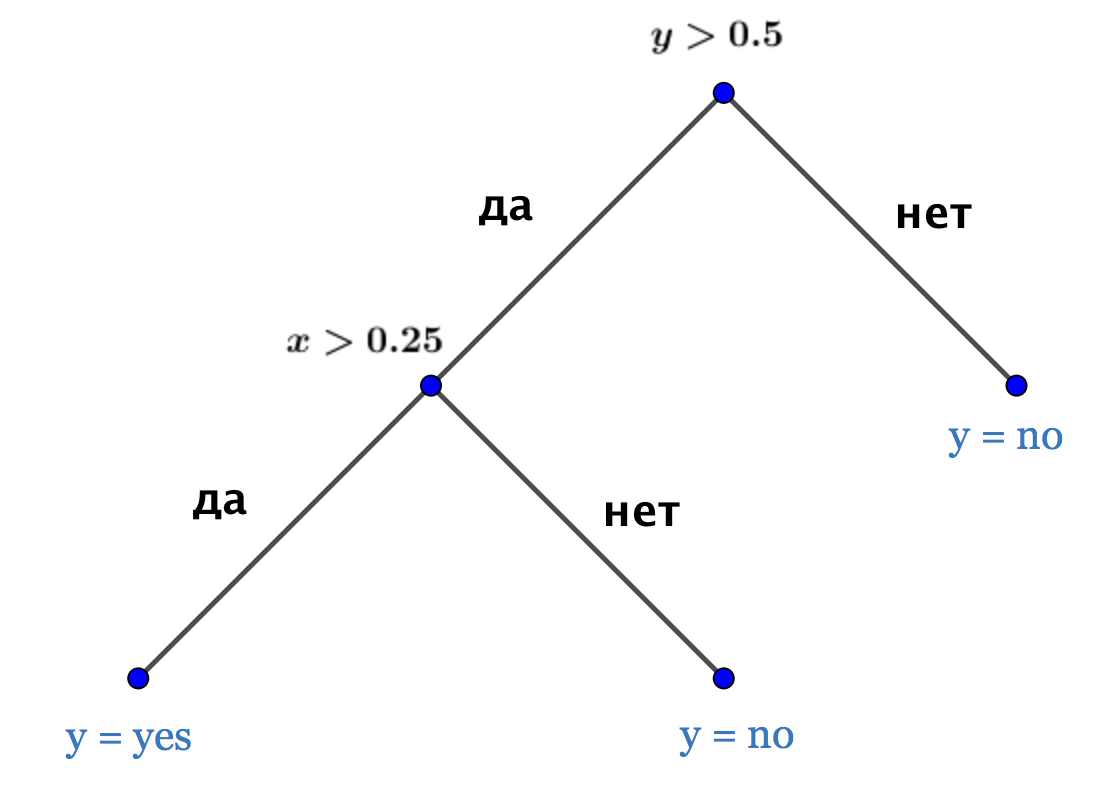
\includegraphics[scale=0.2]{class_tree_3.png}
\end{center} 	
	
Если мы дробим сначала по оси $y$, то мы сразу же довольно сильно уменьшаем неопределённость и ошибаемся только на верхнем левом прямоугольнике, прогнозируя, что он синего цвета. 
	
Если мы дробим сначала по переменной $x$, то мы будем ошибаться на нижнем правом прямоугольнике. Там ошибка намного страшнее. Значит, сначала произойдёт разбиение по $y$, затем по $x$. Именно в этом состоит жадная процедура обучения дерева: уменьшить ошибку при каждом разбиении как можно сильнее. 
\end{solution}

\begin{problem}{}
Рассмотрим обучающую выборку для прогнозирования $y$ с помощью $x$ и $z$:

\begin{center}
	\begin{tabular}{c|c|c}
		$y_i$ & $x_i$ & $z_i$ \\
		\hline
		$y_1$ & $1$ & $2$ \\
		$y_2$ & $1$ & $2$ \\
		$y_3$ & $2$ & $2$ \\
		$y_4$ & $2$ & $1$\\
		$y_5$ & $2$ & $1$ \\
		$y_6$ & $2$ & $1$ \\
		$y_7$ & $2$ & $1$ \\
	\end{tabular}
\end{center}

Будем называть деревья разными, если они выдают разные прогнозы на обучающей выборке. Сколько существует разных классификационных деревьев  для данного набора данных?
\end{problem}

\begin{solution}
Либо мы сначала дробим по $x$, потом по $z$. Либо наоборот. 	\end{solution}

\end{document}